%% LaTeX2e class for student theses
%% thesis.tex
%% 
%% Karlsruhe Institute of Technology
%% Institute for Program Structures and Data Organization
%% Chair for Software Design and Quality (SDQ)
%%
%% Dr.-Ing. Erik Burger
%% burger@kit.edu
%%
%% See https://sdqweb.ipd.kit.edu/wiki/Dokumentvorlagen
%%
%% Version 1.3.5, 2020-06-26

%% Available page modes: oneside, twoside
%% Available languages: english, ngerman
%% Available modes: draft, final (see README)
\documentclass[twoside, english]{sdqthesis}

%% ---------------------------------
%% | Information about the thesis  |
%% ---------------------------------

%% Name of the author
\author{Florian Krone}

%% Title (and possibly subtitle) of the thesis
%\title{Safe Transfer Reinforcement Learning in Changing Environments with High Dimensional Sensor Observations}
\title{Safe Transfer Learning for Robotic Environments}

%% Type of the thesis 
\thesistype{Master's Thesis}

%% Change the institute here, ``IPD'' is default
% \myinstitute{Institute for \dots}

%% You can put a logo in the ``logos'' directory and include it here
%% instead of the SDQ logo
% \grouplogo{myfile}
%% Alternatively, you can disable the group logo
% \nogrouplogo

%% The reviewers are the professors that grade your thesis
\reviewerone{Prof. Dr. Ralf Reussner}
\reviewertwo{Prof. Dr. J. Marius Zöllner}

%% The advisors are PhDs or Postdocs
\advisorone{M.Sc. Karam Daaboul}
%% The second advisor can be omitted
\advisortwo{M.Sc. Jakob Weinland}

%% Please enter the start end end time of your thesis
\editingtime{23. June 2022}{23. December 2022}

\settitle

%% --------------------------------
%% | Settings for word separation |
%% --------------------------------

%% Describe separation hints here.
%% For more details, see 
%% http://en.wikibooks.org/wiki/LaTeX/Text_Formatting#Hyphenation
\hyphenation{
% me-ta-mo-del
}

%% --------------------------------
%% | Bibliography                 |
%% --------------------------------

%% Use biber instead of BibTeX, see README
\usepackage[citestyle=numeric,style=numeric,backend=biber]{biblatex}
\addbibresource{references.bib}

%% ---------------------------------
%% | Imports                       |
%% ---------------------------------
\usepackage{tikz}
\usetikzlibrary{positioning}
\usetikzlibrary{shapes.geometric}
\usetikzlibrary{calc}
\usepackage[ruled, vlined, linesnumbered]{algorithm2e}
\usepackage{subcaption}
\usepackage{multirow}
\usepackage{makecell}
\usepackage{xurl}

%% ---------------------------------
%% | Commands                      |
%% ---------------------------------

\newtheorem{definition}{Definition} \numberwithin{definition}{chapter}
\newtheorem{theorem}[definition]{Theorem}
\newtheorem{lemma}[definition]{Lemma}
\newtheorem{corollary}[definition]{Corollary}
\newtheorem{conjecture}[definition]{Conjecture}

%% ====================================
%% ====================================
%% ||                                ||
%% || Beginning of the main document ||
%% ||                                ||
%% ====================================
%% ====================================
\begin{document}

%% Set PDF metadata
\setpdf

%% Set the title
\maketitle

%% The Preamble begins here
\frontmatter

%% LaTeX2e class for student theses: Declaration of independent work
%% sections/declaration.tex
%% 
%% Karlsruhe Institute of Technology
%% Institute for Program Structures and Data Organization
%% Chair for Software Design and Quality (SDQ)
%%
%% Dr.-Ing. Erik Burger
%% burger@kit.edu
%%
%% Version 1.3.5, 2020-06-26

\thispagestyle{empty}
\null\vfill
\noindent\hbox to \textwidth{\hrulefill} 
\iflanguage{english}{I declare that I have developed and written the enclosed
thesis completely by myself, and have not used sources or means without
declaration in the text.}%
{Ich versichere wahrheitsgemäß, die Arbeit
selbstständig angefertigt, alle benutzten Hilfsmittel vollständig und genau
angegeben und alles kenntlich gemacht zu haben, was aus Arbeiten anderer
unverändert oder mit Änderungen entnommen wurde.}
 
 
%% ---------------------------------------------
%% | Replace PLACE and DATE with actual values |
%% ---------------------------------------------
\textbf{Karlsruhe, 12. December 2022}
\vspace{1.5cm}
 
\dotfill\hspace*{8.0cm}\\
\hspace*{2cm}(\theauthor) 
\cleardoublepage

\setcounter{page}{1}
\pagenumbering{roman}

%% ----------------
%% |   Abstract   |
%% ----------------
 
%% For theses written in English, an abstract both in English
%% and German is mandatory.
%%
%% For theses written in German, a German abstract is sufficient.
%%
%% The text is included from the following files:
%% - sections/abstract

\includeabstract

%% ------------------------
%% |   Table of Contents  |
%% ------------------------
\tableofcontents

\listoffigures
\listoftables

%% -----------------
%% |   Main part   |
%% -----------------

\mainmatter

\chapter{Introduction}
\label{ch:Introduction}

Learning through interaction, this is the paradigm that is usually used to describe reinforcement learning (RL). An agent interacts with an environment and receives a reward signal for its actions. The agent then learns to maximize the reward signal. This basic idea behind reinforcement learning is derived from the way humans learn. \cite{suttonReinforcementLearningIntroduction2018}
At least, this is what is often used to motivate reinforcement learning. However, this explanation forgets an essential part of the learning process. A child does not just start to speak because it taught itself to do so but imitates its parents. Thus the parents act as a teacher for the child. For more complex tasks, we actually employ teachers. Be it in school, or as driving instructors, for example. We do not just learn to drive a car but someone tells us how to do so. Although we might be able to learn how to drive purely from experience, it would be a massive security risk.

With this in mind, reinforcement learning clearly lacks the notion of a teacher. We expect an RL agent to learn complex tasks purely through interaction. In this work, we explore the possibility of extending the reinforcement learning framework with a teacher. The teacher is hidden behind a simple interface. This allows us to develop our approach agnostic to the actual teacher used in practice.

Obviously, a teacher requires knowledge about the task and how to solve it. A possible, yet very simple, the teacher can be designed around a human as a source of knowledge. However, RL algorithms tend to require a lot of samples to learn complex tasks, making this approach very tedious. Another possibility is to utilize another control algorithm, like trajectory optimization, as a teacher. Even other RL agents can be used as teachers.

One might question the need to train an RL agent using a teacher, if we already have a teacher at hand that can solve the same task. The motivation to train the RL agent is manifold. The teacher may only be able to solve a sub-task of the task the RL agent is trained on. The teacher can then still be used to guide the exploration of the RL agent. Another option is to use a different observation for the teacher and the student. If the student uses only images as observation, only a camera is needed as a sensor when using the agent in practice. To help the training, the teacher may use the information from additional sensors. This makes it cheaper to use the student in practice than the teacher. But even if the student and the teacher use the same observations to solve the same task, we benefit from having an RL agent. With modern RL algorithms, we get a stochastic policy that can adapt to changes in the environment. Also, the continued interaction with the environment when using the student in practice can be used to train the agent without a teacher further.

Typically, reinforcement learning aims to solve a task by maximizing a reward function. Additionally, a second goal arises when applying reinforcement learning to real-world problems, especially robotic tasks like those considered in this work. The agent needs to interact with its environment safely. A very obvious safety risk lies in the interaction with humans for a robotic control task. The robot should never harm a human. The second contribution of this work is the development of two novel algorithms to train an agent so that it can be safely used in real-world scenarios.

The remainder of this work is structured as follows. In chapter \ref{ch:preliminaries} we establish the background needed for this work. This includes reinforcement learning in general and the specific algorithms used in his work. Following the preliminaries, we give an overview of related works in chapter \ref{ch:relatedWork}. Chapter \ref{ch:algorithm} first introduces the aforementioned teacher in the preference reward algorithm. Afterward, we propose two novel algorithms for safe RL, safety training, and safety evaluation. All algorithms are evaluated in chapter \ref{ch:experiments} with many experiments on three robotic control environments. We conclude in chapter \ref{ch:Conclusion} with a summary of the approaches and the results. Additionally, we give an outlook on possible future steps.
\chapter{Preliminaries}
\label{ch:preliminaries}

\section{Reinforcement Learning}
\label{sec:preliminaries:rl}

In reinforcement learning (RL) an agent that interacts with an environment is trained to maximize a reward function. The agent takes actions based on observations from the environment. The problem is often formulated as a Markov decision process (MDP). The notation in the following sections is taken from OpenAI Spinning Up \cite{WelcomeSpinningDeep}.

\subsection{Markov Decision Process}
\label{sec:preliminaries:rl:mdp}
\begin{definition}
    \label{def:mdp}
    Given a
    \begin{itemize}
        \item Set of states \emph{S}
        \item Set of actions \emph{A}
        \item Transition probability function $\emph{P}:S\times A\times S \rightarrow [0,1]$
        \item Reward function $\emph{R}: S\times A\times S \rightarrow [0,1]$
        \item Start state distribution $\rho_0$
        \item Discount factor $\gamma$
    \end{itemize}
    the tuple $(S, A, P, R, \rho_0, \gamma)$ is called a Markov decision process (MDP).
\end{definition}
A trajectory $\tau$ is a sequence of states and actions $\tau = (s_0, a_0, s_1, a_1, \dots)$. At a discrete time step $t$, the transition function $P(s'|s,a)=P(s_{t+1}=s'|s_t=s, a_t=s)$ is given by the probability of reaching state $s_{t+1}$ if the current state is $s_t$ and action $a_t$ is taken. According to the Markov property the next state $s_{t+1}$ only depends on the current state $s_t$ and action $a_t$.

The reward function $r_t = R(s_t, a_t, s_{t+1})$ describes the reward for a state-action-next-state triplet. $R$ also denotes the return of a trajectory, given by the discounted sum of rewards:
\begin{equation}
    R(\tau) = \sum^\infty_{t=0} \gamma^t r_t
    \label{eq:trajectory-return}
\end{equation}
The discount factor $\gamma$ describes how import rewards in the future are in contrast to immediate rewards.

Most of the agents in this work do not use the states of the environment as observations, but an image of the environment. In this case the MDP is considered to be partially observable, as not all state information might be observable at every time step.


\subsubsection{Constrained Markov Decision Process}
\label{sec:preliminaries:rl:cmdp}

Multiple definitions of constrained Markov decision processes (CMDP) exist. In this work a CMDP is a MDP extended with a cost function $C:S\times A\times S \rightarrow [0,1]$ and a threshold $\delta \in \mathbb{R}_{\geq 0}$.
Similar to the reward in equation \ref{eq:trajectory-return}, this can be extended for a trajectory:
\begin{equation}
    C(\tau) = \sum^\infty_{t=0} \gamma^t c_t
    \label{eq:trajectory-cost}
\end{equation}
with $c_t = C(s_t,a_t,c_{t+1})$ denoting the cost of a state-action-next-state triplet in a trajectory $\tau = (s_0, a_0, s_1, a_1, \dots)$.
If $C(\tau) \leq \delta$ the trajectory $\tau$ fulfills the constraint.

\subsection{The Reinforcement Learning Goal}
\label{sec:preliminaries:rl:rl-goal}

The agent selects which action to take in the environment based on a policy $\pi$. RL aims to find the policy that maximizes the expected reward. Only stochastic policies $\pi(a|s)$ are used in this work. For a state $s_t$, an action $a_t$ can be sampled from the policy: $a_t \sim \pi(\cdot|s_t)$. In the following, if the state is evident from the context, this will be written as $a\sim\pi$. When combined with the transition probability function, it is also possible to sample whole trajectories $\tau\sim\pi$.

Given the transition probability function $P$, the reward function $R$, and a policy $\pi$, the probability of a trajectory $\tau$ of length $T$ can be written as:
\begin{equation}
    P(\tau|\pi) = \rho_0(s_0)\prod^{T-1}_{t=0}P(s_{t+1}|s_t,a_t)\pi(a_t|s_t)
\end{equation}
The expected return $J_R(\pi)$ when using the policy $\pi$ can then be written as:
\begin{equation}
    J_R(\pi) = \int_\tau P(\tau|\pi)R(\tau) = \underset{\tau \sim \pi}{\mathbb{E}} [R(\tau)]
    \label{eq:trajectory-expected-return}
\end{equation}
The goal of RL, finding the optimal policy $\pi^*$ that maximizes the expected reward, can then be denoted as:
\begin{equation}
    \pi^* = \underset{\pi}{\arg\max} ~J_R(\pi)
    \label{eq:optimal-policy-simple}
\end{equation}
Combining equations \ref{eq:trajectory-return}, \ref{eq:trajectory-expected-return}, and \ref{eq:optimal-policy-simple} yields:
\begin{equation}
    \pi^* = \underset{\pi}{\arg\max} \underset{\tau\sim\pi}{\mathbb{E}}\Big[\sum^\infty_{t=0}\gamma^t R(s_t,a_t,s_{t+1})\Big]
    \label{eq:optimal-policy}
\end{equation}
For a CMDP the expected cost when using policy $\pi$ can be written as:
\begin{equation}
    J_C(\pi) = \int_\tau P(\tau|\pi)C(\tau) = \underset{\tau \sim \pi}{\mathbb{E}} [C(\tau)]
\end{equation}
This changes the RL goal for a CMDP to:
\begin{equation}
    \pi^* = \underset{\pi}{\arg\max} ~J_R(\pi),~ s.t.~ J_C(\pi) \leq \delta
\end{equation}

\subsection{Value Functions}
\label{sec:preliminaries:rl:valueFunctions}

The value of a state $s$ or a state-action pair $(s, a)$ under policy $\pi$ can be represented as the expected return when starting in $s$ and following policy $\pi$. In the case of a state-action pair, the initial action is specified as $a$:
\begin{equation}
    V^\pi(s)=\underset{\tau\sim\pi}{\mathbb{E}}[R(\tau)|s_0=s]
\end{equation}
\begin{equation}
    Q^\pi(s,a)=\underset{\tau\sim\pi}{\mathbb{E}}[R(\tau)|s_0=s, a_0=a]
\end{equation}
If all actions are chosen by the optimal policy, the value functions are denoted in the following way:
\begin{equation}
    V^*(s)=\underset{\pi}{\max}\underset{\tau\sim\pi}{\mathbb{E}}[R(\tau)|s_0=s]
\end{equation}
\begin{equation}
    Q^*(s,a)=\underset{\pi}{\max}\underset{\tau\sim\pi}{\mathbb{E}}[R(\tau)|s_0=s, a_0=a]
\end{equation}
Based on the value functions, the Bellman equations can be formulated. They reformulate the value functions as the sum of the reward we expect to get for being in a state $s$ and the expected return from the next state $s'$, discounted by $\gamma$.

%The Bellman equations, which express the value functions as the sum of the reward expected in a state $s$ and the discounted expected return from the next state $s'$, can be derived from the value functions. These equations take the form:

\begin{equation}
    V^\pi(s)=\underset{\begin{subarray}{c}
        a\sim\pi\\
        s'\sim P(\cdot|s,a)
    \end{subarray}}{\mathbb{E}}[R(s,a,s')+\gamma V^\pi(s')]
\end{equation}
\begin{equation}
    Q^\pi(s,a)=\underset{s'\sim P(\cdot|s,a)}{\mathbb{E}}[R(s,a,s')+\gamma \underset{a'\sim\pi}{\mathbb{E}}[Q^\pi(s',a')]]
\end{equation}
Again, when following the optimal policies, this changes to:\begin{equation}
    V^*(s)=\underset{a}{\max}\underset{s'\sim P(\cdot|s,a)}{\mathbb{E}}[R(s,a,s')+\gamma V^*(s')]
\end{equation}
\begin{equation}
    Q^*(s,a)=\underset{s'\sim P(\cdot|s,a)}{\mathbb{E}}[R(s,a,s)+\gamma \underset{a'}{\max}[Q^*(s',a')]]
\end{equation}


\subsection{Soft Actor-Critic}
\label{sec:preliminaries:rl:sac}

Soft Actor-Critic (SAC) \cite{haarnojaOffPolicyMaximumEntropy} is one of the current state of the art RL algorithms. SAC uses entropy regularization to prevent the policy from only learning a single solution to the problem.
\begin{definition}
    Given a random variable $X$, distributed according to $P$, the \emph{entropy} is given by:
    \begin{equation}
        H(P) = \underset{X\sim P}{\mathbb{E}}[-\log P(X)]
    \end{equation}
\end{definition}

The entropy of the policy is used to change the definition of the optimal policy from equation \ref{eq:optimal-policy}, as well as the value functions and bellman equations, to a trade-off between maximizing the return and the entropy of the policy. A parameter $\alpha$ is added to determine the importance of the entropy.
\begin{equation}
    \pi^* = \underset{\pi}{\arg\max} \underset{\tau\sim\pi}{\mathbb{E}}\Big[\sum^\infty_{t=0}\gamma^t \Big(R(s_t,a_t,s_{t+1}) + 
    \alpha H(\pi(\cdot|s_t))\Big)\Big]
    \label{eq:sac-optimal-policy}
\end{equation}
Therefore, also the value functions change:
\begin{equation}
    V^\pi(s)=\underset{\tau\sim\pi}{\mathbb{E}}\Big[\sum^\infty_{t=0}\gamma^t \Big(R(s_t,a_t,s_{t+1}) + 
    \alpha H(\pi(\cdot|s_t))\Big)\Big|s_0=s\Big]
\end{equation}
\begin{equation}
    Q^\pi(s,a)=\underset{\tau\sim\pi}{\mathbb{E}}\Big[\sum^\infty_{t=0}\gamma^t R(s_t,a_t,s_{t+1}) + 
    \alpha \sum^\infty_{t=1}\gamma^t H(\pi(\cdot|s_t))\Big|s_0=s, a_0=a\Big]
\end{equation}
As well as the Bellman equations. However, the state bellman equation is not needed for SAC. It is therefore omitted here.
\begin{align}
    Q^\pi(s,a) &= \underset{s'\sim P(\cdot|s,a)}{\mathbb{E}}\Big[R(s,a,s') + \gamma\underset{a'\sim\pi}{\mathbb{E}}\Big[Q^\pi(s',a') + \alpha H(\pi(\cdot|s'))\Big]\Big]
    \label{eq:sac-bellman-q-1}\\
    &= \underset{\begin{subarray}{c}
        s'\sim P(\cdot|s,a)\\
        a'\sim\pi
    \end{subarray}}{\mathbb{E}}\Big[R(s,a,s') + \gamma\Big(Q^\pi(s',a') + \alpha H(\pi(\cdot|s'))\Big)\Big]
    \label{eq:sac-bellman-q-2}\\
    &= \underset{\begin{subarray}{c}
        s'\sim P(\cdot|s,a)\\
        a'\sim\pi
    \end{subarray}}{\mathbb{E}}\Big[R(s,a,s') + \gamma\Big(Q^\pi(s',a') - \alpha \log\pi(a'|s')\Big)\Big]
    \label{eq:sac-bellman-q-3}
\end{align}
In newer implementations of SAC, $\alpha$ is often learned during training. \cite{haarnojaLearningWalkDeep2019}

SAC is an off-policy method. This means that when executing an action in the environment, the resulting quintuple \emph{state, action, reward, next state, done} $(s,a,r,s',d)$ is not used for training directly, but stored in a replay buffer $D$. The flag $done$ identifies, whether the episode was terminated after this action.

A SAC implementation consists of an actor, i.e. the policy $\pi_\theta$ and a critic, which in turn consists of two Q-functions $Q_{\phi_i}$ $i \in \{1,2\}$. The double-Q trick helps to make the training more robust. All three components are separate neural networks. $\theta$ and $\phi_i$ denote the parameters of the networks. For a training step, a batch of $(s,a,r,s',d)$ transitions is sampled from the replay buffer.

\subsubsection{Training the Critic}
\label{sec:preliminaries:rl:sac-critic}
Since the Q-function as denoted in equation \ref{eq:sac-bellman-q-3} is an expectation, it can be approximated using samples. For a given sample $(s,a,r,s',d)$ from the replay buffer $D$, only the next action $a'$ needs to be sampled from $\pi(\cdot|s')$:
\begin{equation}
    Q^\pi(s,a) \approx r+\gamma(Q^\pi(s',a')-\alpha \log~ \pi(a'|s')),~ a'\sim\pi(\cdot|s')
    \label{eq:q-approx}
\end{equation}
In practice, this is used to create a target to train the Q-functions:
\begin{equation}
    y(r,s',d) = r+\gamma(1-d)\Big(\underset{j=1,2}{\min}Q_{\overline{\phi}_i}(s',a')-\alpha \log~ \pi_\theta(a'|s')\Big),~ a'\sim\pi_\theta(\cdot|s')
    \label{eq:q-target}
\end{equation}
The recursion in the Bellman equation utilizes two Q-functions parameterized with $\overline{\phi}_i$. These are called the target networks and represent older versions of the two Q-functions whose parameters are updated every few training steps with the new parameters $\phi_i$. The use of target networks stabilizes the training. The policy $\pi_\theta$ is used to sample the following action $a'$. The term $1-d$ is necessary since the episode terminated in case of $d=1$, and there is no return from future actions.

With all this in place, the two Q-functions can be trained using gradient descent with:
\begin{equation}
    J_Q(\phi)_i = \underset{(s,a,r,s',d)\sim D}{\mathbb{E}}\Big[\Big(Q_{\phi_i}(s,a)-y(r,s',d)\Big)^2\Big]
    \label{eq:critic-loss}
\end{equation}

\subsubsection{Training the Actor}
\label{sec:preliminaries:rl:sac-actor}

The goal of SAC is to train a policy that is proportional to the exponential of the Q-function. This results in a stochastic policy that, with a high probability, proposes actions whose Q value is also high for a given state.
\begin{definition}
    For two probability distributions \emph{p, q} on the same probability space $X$, the Kullback-Leibler divergence (KL) \cite{kullbackInformationSufficiency1951} is given by:
    \begin{equation}
        D_{KL}(p||q) = \sum_{x\in X}p(x) \log \frac{p(x)}{q(x)}
    \end{equation}
    The KL is a similarity measure between the two distributions. It is always non-negative and zero if and only if  $p = q$. Nevertheless, it is not symmetric.
\end{definition}
The policy parameters can be optimized by minimizing the KL of the policy and the exponential of the Q-function:
\begin{align}
    & \underset{s\sim D}{\mathbb{E}}\Bigg[D_{KL}\Bigg(\pi_\theta(\cdot|s)\Bigg|\Bigg|\frac{\exp\big(\frac{1}{\alpha}Q_\phi(s,\cdot)\big)}{Z_\phi(s)}\Bigg)\Bigg]\\
    &= \underset{s\sim D}{\mathbb{E}}\Bigg[\sum_{a\in A} \pi_\theta(a|s) \log\Bigg(\frac{\pi_\theta(a|s)Z_\phi(s)}{\exp\big(\frac{1}{\alpha}Q_\phi(s,a)\big)}\Bigg)\Bigg]\\
    &= \underset{\begin{subarray}{c}
        s\sim D\\
        a\sim \pi_\theta(\cdot|s)
    \end{subarray}}{\mathbb{E}}\Big[\log\pi_\theta(a|s)+\log Z_\phi(s)-\frac{1}{\alpha}Q_\phi(s,a)\Big]
    \label{eq:pi-kl-3}
\end{align}
The function $Z_\phi(s)$ is needed to normalize $\exp Q_\phi(s, \cdot)$, since the KL is only defined for two distributions. It was shown that $Z_\phi(s)$ is not present in the gradient with respect to $\theta$. Therefore it is omitted in the future. Additionally the equation is multiplied by $\alpha$ to get the training objective:
\begin{equation}
    J_\pi(\theta) = \underset{\begin{subarray}{c}
        s\sim D\\
        a\sim \pi_\theta(\cdot|s)
    \end{subarray}}{\mathbb{E}}\Big[\alpha\log\pi_\theta(a|s)-Q_\phi(s,a)\Big]
    \label{eq:pi-objective-no-reparam}
\end{equation}
This objective cannot be directly approximated through Monte Carlo estimation, because the the distribution that has to be sampled from depends on the parameters that are to be optimized. However, since the policy is supposed to be a Gaussian, the reparametrization trick can be used. Instead of having a probabilistic neural network for the policy that directly gives an action for each state, a double headed, deterministic network is used. The two heads are the functions $\mu_\theta(s)$ and $\sigma_\theta(s)$. The distribution of actions for each state $s$ is then given by:
\begin{equation}
    f_\theta(s, \xi) = \mu_\theta(s) + \sigma_\theta(s)\xi,~ \xi \sim \mathcal{N}(0, I)
    \label{eq:reparam-trick}
\end{equation}
With this reparametrization, equation \ref{eq:pi-objective-no-reparam} can be rewritten as:
\begin{equation}
    J_\pi(\theta) = \underset{\begin{subarray}{c}
        s\sim D\\
        \xi\sim \mathcal{N}(0, I)
    \end{subarray}}{\mathbb{E}}\Big[\alpha\log\pi_\theta(f_\theta(s, \xi)|s)-Q_\phi(s,f_\theta(s, \xi))\Big]
\end{equation}
Now, the distribution the expectation is taken over no longer depends on $\theta$. Finally, as described in section \ref{sec:preliminaries:rl:sac-critic}, SAC uses two Q-functions to stabilize the training. Therefore, the more pessimistic of the two should be used in the training objective:
\begin{equation}
    J_\pi(\theta) = \underset{\begin{subarray}{c}
        s\sim D\\
        \xi\sim \mathcal{N}(0, I)
    \end{subarray}}{\mathbb{E}}\Big[\alpha\log\pi_\theta(f_\theta(s, \xi)|s)-\underset{i=1,2}{\min}Q_{\phi_i}(s,f_\theta(s, \xi))\Big]
    \label{eq:actor-loss}
\end{equation}
With batches of states drawn from the replay buffer, this objective function is used to optimize the policy using gradient descent.

In practice, the reparametrization trick is extended with a $\tanh$ to ensure that the actions are in a valid range:
\begin{equation}
    f_\theta(s, \xi) = \tanh(\mu_\theta(s) + \sigma_\theta(s)\xi),~ \xi \sim \mathcal{N}(0, I)
\end{equation}

\subsubsection{SAC algorithm}
\label{sec:preliminaries:rl:sac-algo}

The SAC algorithm, outlined in algorithm \ref{alg:sac}, combines the two training objectives. First, the target networks are set to the same parameters as the initial Q-functions. Also the empty replay buffer is initialized and the initial state $s$ is observed from the environment. Afterwards, the training loop starts. First, an action $a$ is sampled from the policy for the current state. This action is executed in the environment returning the reward $r$, next state $s'$ and an indicator if the episode is done $d$. The Quintuple $(s,a,r,s',d)$ is added to the replay buffer. If the episode is done, the environment is reset and the initial state is loaded again. Afterwards, a batch is sampled from the replay buffer and a gradient descent update is done. First, the Q-function targets are calculated according to equation \ref{eq:q-target}. The parameters for the two Q-functions and the policy are updated with the objectives from the equations \ref{eq:critic-loss} and \ref{eq:actor-loss}. Lastly the weights of the target networks are updated.

Variations of this algorithm exist and include mainly different execution frequencies. It is possible to execute multiple environment steps without having a gradient descent in between, or do multiple updates after each environment step. Also the target networks may not be updated after ever step. The algorithm as described here, is the variant that was used during this work.

\begin{algorithm}[btp]
    \caption{Soft Actor-Critic}
    \label{alg:sac}

    \DontPrintSemicolon
    \SetFuncSty{textsc}
    
    \KwIn{entropy coefficient $\alpha$, environment $e$, initial parameters $\theta, \phi_1, \phi_2$, learning rates $\eta_\pi$, $\eta_Q$, target update rate $\rho$}
    \KwData{replay buffer $D$}
    \KwOut{$\theta, \phi_1, \phi_2$}

    \SetKwFunction{append}{append}
    \SetKwFunction{initialstate}{initialState}
    \SetKwFunction{step}{step}
    \SetKwFunction{reset}{reset}
    
    \BlankLine
    \tcp{Initialize target networks}
    $\overline{\phi}_1 \gets \phi_1$, $\overline{\phi}_2 \gets \phi_2$\;
    $s\gets e.\initialstate()$\;
    
    \For{each iteration}{
        \tcp{Interact with the environment}
        $a\sim \pi_\theta(\cdot|s)$\;
        $r, s', d\gets e.\step(a)$\;
        $D.\append((s,a,r,s',d))$\;
        \If{$d = done$}{
            $e.\reset()$\;
            $s\gets e.\initialstate()$\;
        }
        Sample a batch $B$ of transitions from $D$\;
        \tcp{Compute Q-function targets}
        \ForEach{$(s,a,r,s',d)\in B$}{
            $y(r,s',d) \gets r+\gamma(1-d)\Big(\underset{j=1,2}{\min}Q_{\overline{\phi}_i}(s',a')-\alpha \log~ \pi_\theta(a'|s')\Big),~ a'\sim\pi_\theta(\cdot|s')$\;
        }
        \tcp{Update Q-functions and policy by one step of gradient descent}
        \For{$i=1,2$}{
            $\phi_i\gets \phi_i - \eta_Q\nabla_{\phi_i}\frac{1}{|B|} \sum_{(s,a,r,s',d)\in B}\Big[\Big(Q_{\phi_i}(s,a)-y(r,s',d)^2\Big)\Big]$
        }
        \For{$i = 1,2,\dots,|B|$}{
            $\xi_i\gets \mathcal{N}(0,I)$\;
        }
        $\theta\gets \theta - \eta_\pi\nabla_\theta\frac{1}{|B|} \sum_{s\in B}\Big[\alpha\log\pi_\theta(f_\theta(s, \xi_i)|s)-\underset{i=1,2}{\min}Q_{\phi_i}(s,f_\theta(s, \xi_i))\Big]$\;
        \tcp{Update target networks}
        \For{$i=1,2$}{
            $\overline{\phi}_i\gets \rho\overline{\phi}_i + (1-\rho)\phi_i$\;
        }
        return $\theta, \phi_1, \phi_2$\;
    }
\end{algorithm}

\section{High Dimensional Observations}
\label{sec:preliminaries-high-dim-observations}

When talking about high dimensional observations in RL, this usually means images of the environment. This is in contrast the actual state which consists of vectors with the position and velocity of the objects. Since it is not possible to extract the velocity from a single image, it is common practice to use multiple consecutive images as observations \cite{mnihPlayingAtariDeep2013, kostrikovImageAugmentationAll2021, srinivasCURLContrastiveUnsupervised2020, yaratsImprovingSampleEfficiency2020}. This is called a frame stack.

In the first step, the images are converted to a latent space using an encoder. When using SAC, the latent space is then given to the actor and critic networks to produce actions and reward estimates. The only difference between using image and space observations lies in the encoder. State observations can be used directly with the actor and critic networks without the need for an encoder. The encoder consists of a multi layer CNN. The output of the last convolution is flattened to produce a one dimensional vector for the latent space.

Different approaches have been attempted to improve the performance of RL with high dimensional observations. They include auxiliary losses \cite{yaratsImprovingSampleEfficiency2020, stookeDecouplingRepresentationLearning, srinivasCURLContrastiveUnsupervised2020} as well as data augmentations \cite{kostrikovImageAugmentationAll2021}. In this work, autoencoders and DrQ, a data augmentation technique, were used to improve the performance.

An \emph{autoencoder} is a combination of two neural networks, an encoder $f_{enc}: D \rightarrow K$ and a decoder $f_{dec}: K \rightarrow D$. Typically, the latent space $D$ is smaller than the input dimension $K$. With the combination of the encoder and decoder, $z = f_{dec}(f_{enc}(x))$ can be computed. The goal of an autoencoder is that $z \approx x$. A reconstruction loss is used to train the autoencoder self supervised using gradient descent. For an image the reconstruction loss is given by the pixel wise mean square error.
\begin{figure}[btp]
    \centering
        \begin{tikzpicture}
            \node[text width=1cm] (center) {Latent Space};
            \node [left=0.5cm of center, trapezium, draw, thick, shape border rotate=270, trapezium stretches=true, minimum width = 4cm] (encoder) {Encoder};
            \node [right=0.5cm of center, trapezium, draw, thick, shape border rotate=90, trapezium stretches=true, minimum width = 4cm] (decoder) {Decoder};
            \node[left=.2cm of encoder] (original)  {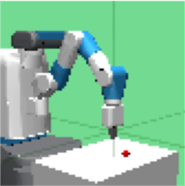
\includegraphics[height=4cm]{images/ae_input.png}};
            \node[right=.2cm of decoder] (recreated) {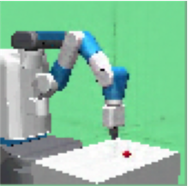
\includegraphics[height=4cm]{images/ae_recreated.png}};
            \node[below=0.5cm of original] (original_text) {Input $x$};
            \node[below=0.5cm of recreated] (recreated_text) {Reconstruction $z = f_{dec}(y)$};
            \node at (0,42 |- original_text) {$y = f_{enc}(x)$};
        \end{tikzpicture}
    \caption[High level view of an autoencoder]{High level view of an autoencoder. The reconstructed image is the actual output from an autoencoder that was trained during this work for the input image.}
    \label{fig:ae-explanation}
\end{figure}
Figure \ref{fig:ae-explanation} visualizes how an autoencoder works.

In RL, autoencoders can be used as an auxiliary loss to enhance the performance of agents trained on pixel observations. \citeauthor{yaratsImprovingSampleEfficiency2020} \cite{yaratsImprovingSampleEfficiency2020} proposed an architecture where a shared CNN feature extractor is trained by the loss of the critic and an reconstruction loss. The feature extractor is also used by the actor network, but detached during training, i.e. no updates are performed on the encoder when training the actor.

\citeauthor{kostrikovImageAugmentationAll2021} \cite{kostrikovImageAugmentationAll2021} investigated the effects of image augmentations on the performance of SAC pixels. Based on this, they developed a regularization approach called Data-regularized Q (DrQ) to enhance performance. Their idea was not simply to train the agent with augmented images but to average the Q-function over $M \geq 1$ different augmentations of the same image. Additionally, they averaged the Q target (equation \ref{eq:q-target}) over $K \geq 1$ different augmentations. A differently positioned random cropping gives the augmentations. All images from the environment have $84\times84$ pixels. First, they are padded by four pixels on each site. As padding, they used the repeated boundary pixels. Then a random crop of size $84\times84$ pixels is selected from the padded image.
\chapter{Related work}
\label{ch:relatedWork}

This work combines  three active fields of research in reinforcement learning (RL), Transfer Learning, Safe RL and the usage of pixel observations. The following sections will provide an overview of different approaches in these fields.

\section{Transfer Learning}
\label{sec:transferLearning}

Transfer learning is very well known in supervised learning. It usually refers to using a pre trained model, or a part of it, and fine tune it on a new problem, reducing the training time on the new problem. This approach has been used for RL as well, for example by \citeauthor{delacruzInitialProgressTransfer2016} \cite{delacruzInitialProgressTransfer2016}. They were able to improve the performance in some Atari games, by transferring some layers from agents, trained on other Atari games. \citeauthor{gamrianTransferLearningRelated2019a} \cite{gamrianTransferLearningRelated2019a} found that an agent trained on the first level of the Nintendo game Road Fighter was not able to complete subsequent levels. However, when mapping the images back to the familiar images from the first level, using GANs, the agent was able to complete the level. Thus, they were able to transfer knowledge from one task to another.

\section{Safe Reinforcement Learning}
\label{sec:safeRL}

\citeauthor{guReviewSafeReinforcement2022} \cite{guReviewSafeReinforcement2022} defined five problems, called \enquote{2H3W}, in safe RL. The problems are safety policy, complexity, applications, benchmarks, and challenges. Our work addresses the safety policy problem, formulated as \enquote{How can we perform policy optimization to search for a safe policy?}\cite{guReviewSafeReinforcement2022} Therefore, this section focuses on solutions for this problem.

Often, the problem is formulated as a Constrained Markov Decision Process (CMDP), as described in Section \ref{sec:preliminaries:rl:cmdp}. From this, a Lagrangian function can be formulated, combining the reward function with the constraints. A number of Algorithms have been proposed to solve a CMDP with this approach \cite{borkarActorcriticAlgorithmConstrained2005, yuConvergentPolicyOptimization2019, tesslerRewardConstrainedPolicy2018, paternainConstrainedReinforcementLearning2019, paternainSafePoliciesReinforcement2022}. \citeauthor{bharadhwajConservativeSafetyCritics2021} \cite{bharadhwajConservativeSafetyCritics2021} combined this approach with a safety critic to estimate the expected cost, similar to our approach. However, they only use the critic during the sampling of actions. Others adapted trust region methods to also consider safety constraints \cite{achiamConstrainedPolicyOptimization2017}. 

A number of algorithms have been developed that attempt to train for reward and safety in different steps. \citeauthor{yangProjectionBasedConstrainedPolicy2020} \cite{yangProjectionBasedConstrainedPolicy2020} build upon TRPO to first learn a policy that optimizes the reward and then projecting it back to the closest policy that fulfills the constraints. Similarly, \citeauthor{wagenerSafeReinforcementLearning2021} \cite{wagenerSafeReinforcementLearning2021} developed an algorithm that is agnostic of the underlying RL algorithm. They learn a policy agnostic of safety, but before executing the actions in the environment, they are run through an intervention policy and potentially changed to ensure safety. A similar approach was followed by \citeauthor{phamOptLayerPracticalConstrained2018} \cite{phamOptLayerPracticalConstrained2018}. They developed an OptLayer, that computes a safe action, closest to the original prediction.  \citeauthor{wachiSafeReinforcementLearning2020} \cite{wachiSafeReinforcementLearning2020} proposed an algorithm that first expands a safety region, and then explores and exploits the region to optimize the reward.

\section{Pixel Observations}
\label{sec:pixelObservations}

Training RL agents on high dimensional image observations has proven to be less sample efficient and the agents are usually performing worse than their counterparts trained on the complete state information \cite{yaratsImprovingSampleEfficiency2020, kostrikovImageAugmentationAll2021, srinivasCURLContrastiveUnsupervised2020}. It is an active field of research, how to close the gap to state based agents.

\citeauthor{kostrikovImageAugmentationAll2021} \cite{kostrikovImageAugmentationAll2021} investigated the effects of image augmentations on the performance and sample efficiency. Additionally, they proposed novel regularization techniques for the target Q and Q function, by averaging over multiple samples, obtained through different augmentations on a single observation.

\citeauthor{yaratsImprovingSampleEfficiency2020} \cite{yaratsImprovingSampleEfficiency2020} used an autoencoder to aid the agents ability to learn a latent space from the pixel observations. Similarly, \citeauthor{srinivasCURLContrastiveUnsupervised2020} \cite{srinivasCURLContrastiveUnsupervised2020} applied a contrastive loss as auxiliary loss to improve the encoder. To do so, they use two encoders, each getting different data-augmented versions of the observation. Based on this, \citeauthor{zhanFrameworkEfficientRobotic2020} \cite{zhanFrameworkEfficientRobotic2020} proposed the FERM architecture, where a replay buffer is initialized with human demonstrations, which are then used to pre-train the encoder, using a contrastive loss. Afterwards, the pre-filled replay buffer and pre-trained encoder are used to train a SAC agent. Again, using contrastive loss, \citeauthor{stookeDecouplingRepresentationLearning} \cite{stookeDecouplingRepresentationLearning} aided the training of the encoder by comparing it to an encoded example from $k$ time steps later.

Lastly, when attempting to train under realistic assumptions, images are not the only possible observation. When using a robot arm, the position of the end-effector can be measured, as well as if its is open. A combination of images and a subspace of the complete state, regarding the robot, has been used by \citeauthor{kalashnikovQTOptScalableDeep2018} \cite{kalashnikovQTOptScalableDeep2018} to train robotic manipulation tasks.
\chapter{Algorithm}
\label{ch:algorithm}

The original goal of the preference reward algorithm was to transfer learned behavior from one RL agent to another. It is, however, designed to only rely on an abstract interface of the source of knowledge, the teacher. A teacher, as described in definition \ref{def:teacher}, if given a state, proposes an action together with a confidence about the quality of this action.
\begin{definition}
    \label{def:teacher}
     Let $(S, A, P, R, \rho_0, \gamma)$ be a MDP. Then a function $$T: S \rightarrow A\times[0,1]$$ is called a \emph{teacher} for this MDP. A teacher proposes an action for each state and gives a confidence about the quality of this action.
\end{definition}
In practice, a teacher does not necessarily has to be a RL agent, but can also be a trajectory planner or other means of solving the task at hand. See section \ref{sec:teachers} about different kinds of teachers. The following section \ref{sec:preference-reward} outlines the preference reward algorithm.

\section{Preference Reward}
\label{sec:preference-reward}

The preference reward algorithm uses reward shaping to assist the exploration of a RL agent in training. It can therefore be used with any RL algorithm. The reward is changed based on the actions that a teacher suggests for the current state. This action is considered the preferred action. See section \ref{sec:teachers} for details about teachers.

Three different rewards are used for an MDP and a teacher $T$, the \emph{environment reward}, \emph{teacher reward} and \emph{preference reward}. See definition \ref{def:preference-reward}. First, the reward from the MDP is called \emph{environment reward} $r_{env}$. For a state $s$ and an action $a$ proposed by the agent, the teacher gives an action $\hat{a}$ and a confidence $c$. The confidence is used by the teacher to rate the quality of its action $\hat{a}$. The mean square error, of $a$ and $\hat{a}$ is called the \emph{action error}. The action error, multiplied with the negated confidence forms the \emph{teacher reward} $r_{teacher}$. The teacher reward may be seen as a penalty for the agent if the proposed actions are not in line with the teachers actions. The confidence makes sure that the penalty is lower if the teacher is not confident about the quality of its action. Lastly, the weighted sum of the environment and teacher reward is called \emph{preference reward} $r_{pr}$. The importance of the teacher reward is determined by a parameter $\alpha \in [0,1]$.
\begin{definition}
    \label{def:preference-reward}
    Let $(S, A, P, R, \rho_0, \gamma)$ be a MDP, $T$ a teacher, $(s, a, s')$ a state, action, next state triplet, and $\alpha \in [0,1]$. Then:
    \begin{enumerate}[(1)]
        \item\label{enm:pr:external-reward} $r_{env} = R(s, a, s')$ is called \emph{environment reward}.
        \item\label{enm:pr:internal-reward} Let $T(s) = (\hat{a}, c)$. Then $r_{teacher} = -c * \frac{1}{dim(A)} \sum_i (a_i - \hat{a}_i)^2$ is called \emph{teacher reward}.
        \item\label{enm:pr:preference-reward} $r_{pr} = \alpha * r_{teacher} + (1-\alpha) * r_{env}$ is called \emph{preference reward}.
    \end{enumerate}
\end{definition}

Algorithm \ref{alg:preference-reward} outlines the steps to calculate the preference reward. First, the teacher is used to obtain the preferred action $\hat{a}$ and the confidence $c$. Together with the action $a$ from the agent, the teacher reward is calculated. Lastly, the preference reward is calculated from the environment reward and the teacher reward.
\begin{algorithm}[btp]
    \caption{Preference Reward}
    \label{alg:preference-reward}

    \DontPrintSemicolon
    \SetFuncSty{textsc}
    
    \KwIn{action $a \in \mathbb{R}^n$, state $s$, reward $r_{env}$, teacher $T$, $\alpha \in [0,1]$}
    \KwData{$\hat{a} \in \mathbb{R}^n$, $c \in \mathbb{R}$, $r_{teacher} \in \mathbb{R}$}
    \KwOut{preference reward $r_{pr} \in \mathbb{R}$}

    \SetKwFunction{predict}{predict}
    \SetKwFunction{random}{selectRandomElement}
    \SetKwFunction{std}{standardDeviation}
    \SetKwFunction{exp}{exp}
    
    \BlankLine
    $\hat{a}, c \leftarrow T(s, a)$\;
    $r_{teacher}\leftarrow -c * \frac{1}{n} \sum_{i=0}^n(a_i-\hat{a}_i)^2$\;
    $r_{pr}\leftarrow \alpha * r_{teacher} + (1-\alpha) * r_{env}$\;
    return $r_{pr}$\;
\end{algorithm}

\subsection{Adaptive Alpha}
\label{sec:adaptive-alpha}

The parameter $\alpha$ that determines the importance of the preference reward does not necessarily need to be a fixed value. It is possible to change the value of $\alpha$ based on different factors. In fact, it turned out to increase the success rate of the agent, to reduce the $\alpha$ value as the training progressed. See the experiment results in section \ref{sec:experiments:results}. We explored two methods for adapting $\alpha$ during training: one based on the number of training steps completed, and another based on the rewards our agent was receiving in its environment

For an adaptive $\alpha$ based on training steps, the $\alpha$ with a value of one and is linearly reduced to zero at the final training step. The adaptive $\alpha$ based on the environment reward assumes that the agent is getting better if the environment reward increases and therefore does not need as much guidance from the teacher. To make the $\alpha$ value more stable, we used an exponential moving average of the environment reward to calculate it.

Other options to adapt $\alpha$ are possible, but we leave them for future work.

\subsection{High Dimensional Observations}
\label{sec:algo-high-dim-observations}

In this work, the preference reward algorithm was used to assist the training of a SAC agent using high dimensional image observations, assuming that during training, the full state of the environment is available. Figure \ref{fig:algorithm} shows the training setup. The SAC agent only relies on a frame stack as observations, the state is only needed for the teacher during training. Optionally, the gripper position can be added to the observation, to simplify the task. The gripper position could be obtained from a real world robot and does therefore not break the goal to train under realistic assumptions.

The idea behind this setup is to utilize more information during training than during evaluation. In a real world application, this would result in using more sensors during training to measure the state of the environment and use it for the teacher. But during evaluation, the trained agent only relies on simple sensor data, such as images and the gripper position.

\begin{figure}[btp]
    \centering
    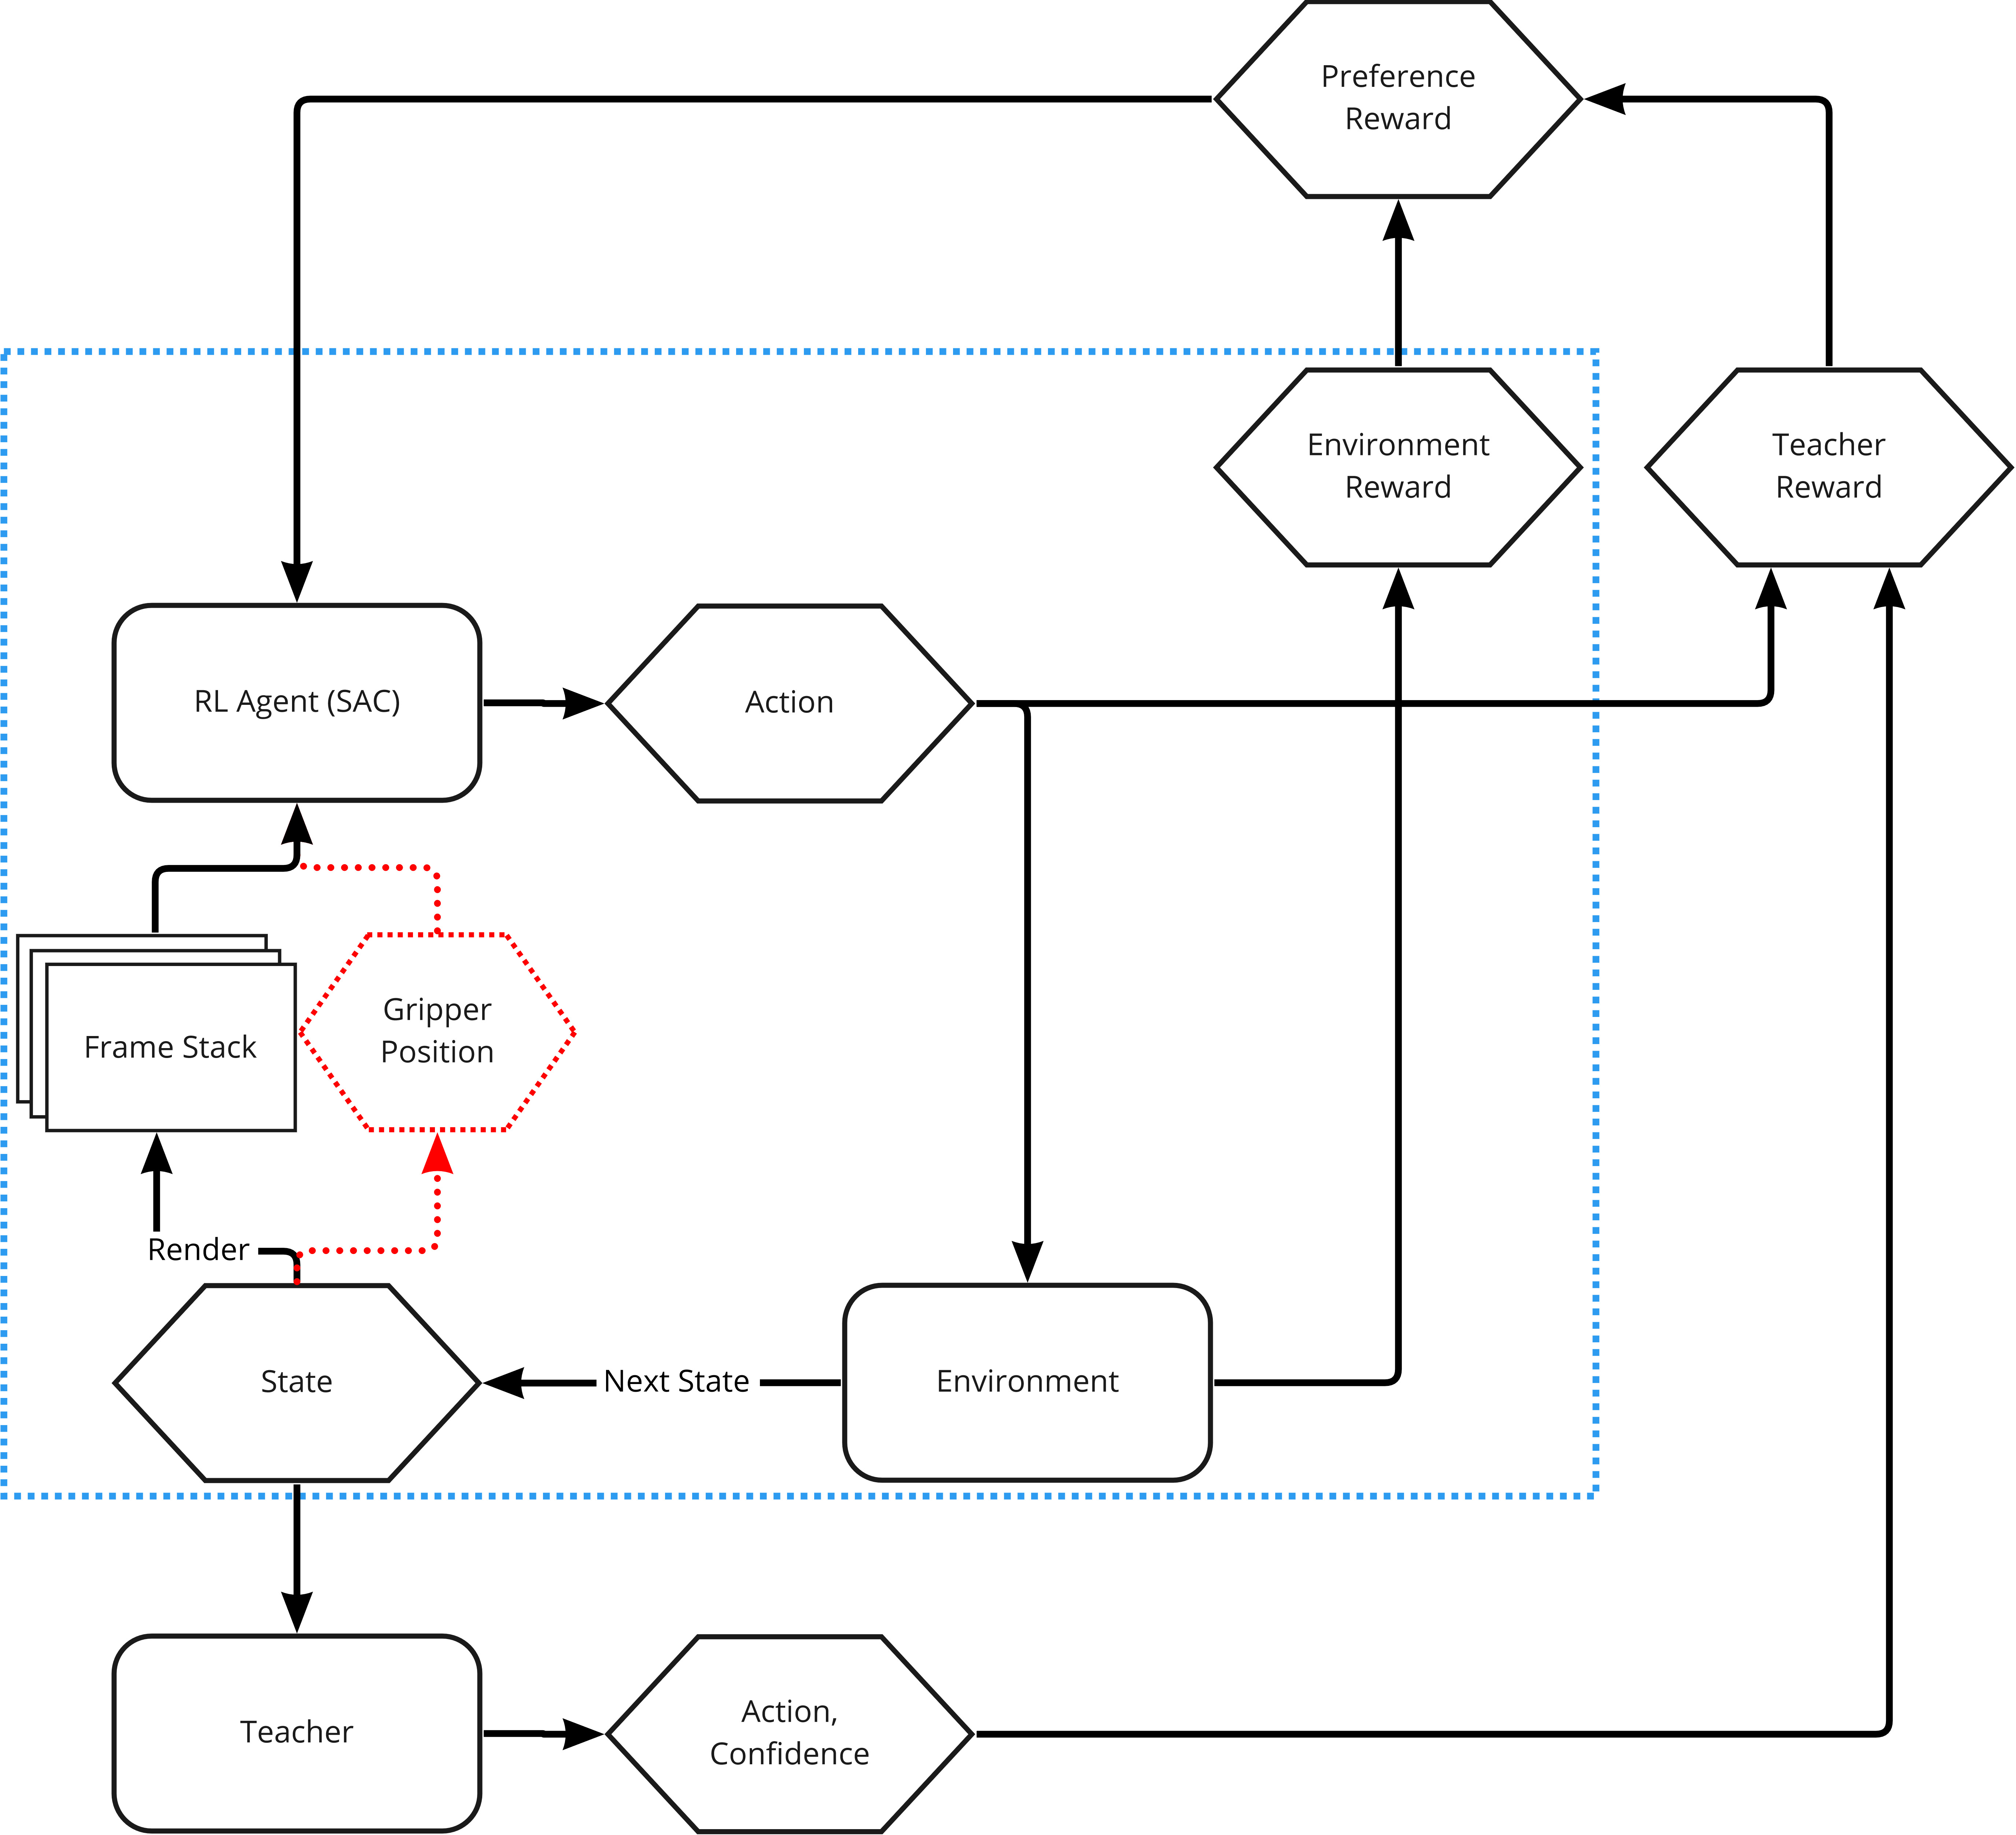
\includegraphics[width=\textwidth]{images/algorithm.jpg}
    \caption[Overview of the preference reward algorithm]{Overview of the preference reward algorithm to train an agent on high dimensional image observations. Optionally, the gripper position of a robot can be added to the observation. The elements marked in blue are present in regular SAC.}
    \label{fig:algorithm}
\end{figure}

\subsection{Teachers}
\label{sec:teachers}

As stated in definition \ref{def:teacher}, a teacher is a function that proposes an action for each state and provides a confidence about the quality of this action. For the training setup as described in section \ref{sec:algo-high-dim-observations}, the teacher may use a RL agent trained on the full state of the environment to obtain the preferred action. To obtain the confidence, algorithm \ref{alg:ensemble-teacher} uses an ensemble of multiple teachers. First, the element wise standard deviation is calculated. Then the exponential of the negative standard deviation is used as confidence, to ensure a range of $[0,1]$. From the actions proposed by the agents of the ensemble, one is drawn at random as the preferred action. Note that in this case, the teacher is not a mathematical function, as it is not deterministic. Another way to obtain the confidence with just a single agent is to use dropout as Bayesian approximation, as described in \cite{galDropoutBayesianApproximation2016}.

The training setup described in section \ref{sec:algo-high-dim-observations} and figure \ref{fig:algorithm} is not the only setup where a RL agent can be used as a teacher. In a slightly modified version of this setup, where the teacher and the student both receive the same observation, it is still possible to utilize an RL agent as a teacher. While the teacher would not be able to solve the task at hand perfectly, it could be an agent that can solve a simpler sub task and therefore guide the exploration of the agent in training.

However, the teacher does not necessarily has to be an RL agent. Other means to propose an action may be used as teachers as well. They only need to fulfill definition \ref{def:teacher}, that is being able to provide an action and a confidence for each state. One example would be a trajectory planner.

\begin{algorithm}[btp]
    \caption{Ensemble Teacher}
    \label{alg:ensemble-teacher}

    \DontPrintSemicolon
    \SetFuncSty{textsc}
    
    \KwIn{action $a \in \mathbb{R}^n$, state $s$, list of RL agents $L$}
    \KwData{list of actions $A$}
    \KwOut{action $\hat{a} \in \mathbb{R}^n$, confidence $c \in [0,1]$}

    \SetKwFunction{append}{append}
    \SetKwFunction{predict}{getAction}
    \SetKwFunction{random}{selectRandomElement}
    \SetKwFunction{std}{standardDeviation}
    \SetKwFunction{exp}{exp}
    
    \BlankLine
    \tcp{L is only provided when initializing the teacher and not each time}
    \ForEach{$agent$ in $L$}
    {$A$.\append(agent.\predict(s))}
    $\hat{a} \leftarrow\random{A}$\;
    $c \leftarrow\exp(-\std(A))$\;
    return $\hat{a}, c$\;
\end{algorithm}

\section{Safety}
\label{sec:safety}

As described in section \ref{sec:preliminaries:rl:cmdp}, a constrained Markov decision process is a MDP extended by a cost function $C(s,a,s')\rightarrow[0,1]$ and a threshold $\delta \in \mathbb{R}_{\geq 0}$. Three different approaches were attempted in this work to extend SAC to CMDPs. The goal with these was not to strictly stay below the threshold $\delta$, but to learn a policy that minimizes the expected cost of an episode. One of the approaches uses reward shaping and the other two a safety critic.

\subsection{Reward Based}
\label{sec:reward-based}

The first, and simplest approach is to penalize the agent by deducting the cost of a state, action, next state triplet $(s, a, s')$ from the reward:
\begin{equation}
    \label{eq:reward-based-cost}
    R_{cost}(s,a,s') = \lambda_r R(s,a,s') - \lambda_c C(s,a,s')
\end{equation}
The parameters $\lambda_r, \lambda_c \geq 0$ symbolize the importance of the reward and the cost. With this approach, the new reward function $R_{cost}$ is not guaranteed to be in the interval $[0,1]$.

\subsection{Safety Critic}
\label{sec:safety-critic}

The cost is defined in the same way as the reward, the only difference is that the goal is to minimize the cost while the reward should be maximized. It is therefore possible to formulate the value functions and bellman equations $V^\pi(s)$ and $Q^\pi(s,a)$ just like in section \ref{sec:preliminaries:rl:valueFunctions}. In the following, an index $R$ or $C$ is added to the functions to indicate whether they are the reward or safety function. The parameter vectors for the Q-function neural networks are indexed in the same way as $\phi^C_i$ and $\phi^R_i$, where $i$ is the index for the double-Q trick. 

The functions for the optimal policy $V_C^*(s)$ and $Q_C^*(s,a)$ can not be formulated just like that, because the goal is not to minimize the cost but to maximize the reward while maintaining a low cost. It is therefore not clearly defined what the optimal policy is. The same is true for the reward function regarding the optimal policy $V_R^*(s)$ and $Q_R^*(s,a)$. This is, however, not a problem, since the optimal policy functions are not needed for SAC.

Together with the entropy, this results in the following cost Bellman equation similar to equation \ref{eq:sac-bellman-q-3}:
\begin{equation}
    Q_C^\pi(s,a) = \underset{\begin{subarray}{c}
        s'\sim P(\cdot|s,a)\\
        a'\sim\pi
    \end{subarray}}{\mathbb{E}}\Big[C(s,a,s') + \gamma\Big(Q_C^\pi(s',a') - \alpha \log\pi(a'|s')\Big)\Big]
    \label{eq:sac-cost-bellman}
\end{equation}

During training, the replay buffer also stores the cost of a transition. A sample from it is therefore a sextuple $(s,a,r,c,s',d)$, where c denotes $C(s,a,s')$. With this, similar to equation \ref{eq:q-approx}, the safety-Q can be approximated:
\begin{equation}
    Q_C^\pi(s,a) \approx c+\gamma(Q_C^\pi(s',a')-\alpha \log~ \pi(a'|s')),~ a'\sim\pi(\cdot|s')
    \label{eq:safety-q-approx}
\end{equation}
Again, this is used to create the target function:
\begin{equation}
    y_C(c,s',d) = c+\gamma(1-d)\Big(\underset{j=1,2}{\max}Q_{\overline{\phi}^C_i}(s',a')-\alpha \log~ \pi_\theta(a'|s')\Big),~ a'\sim\pi_\theta(\cdot|s')
    \label{eq:safety-q-target}
\end{equation}
Just like for the reward critic, older versions of the two Q-functions are used to calculate the target. This stabilizes the training. They are denoted with ${\overline{\phi}^C_i}$. Note that in contrast to equation \ref{eq:q-target} the maximum of the two Q-functions is used.
Just like the reward critic, the safety critic can be trained with:
\begin{equation}
    J_{Q_C}(\phi)_i = \underset{(s,a,r,c,s',d)\sim D}{\mathbb{E}}\Big[\Big(Q_{\phi^C_i}(s,a)-y_C(c,s',d)\Big)^2\Big]
\end{equation}

In this work, two different ways to use the safety critic were evaluated. One is to use the safety critic during the training of the policy. The other approach only uses the safety critic in the evaluation.

\subsubsection{Safety Training}
\label{sec:safety-training}

The first approach using the safety critic changes the training objective of the actor. Instead of training an actor that is proportional to the exponential of the Q-function, it should now be proportional to the difference between the reward and safety critic:
\begin{equation}
    \pi(a| s) \propto \exp(Q_R(s, a) - Q_C(s,a))
\end{equation}
This also changes the goal to minimize the Kullback-Leibler divergence between the actor and the exponential difference between the two critics:
\begin{align}
    & \underset{s\sim D}{\mathbb{E}}\Bigg[D_{KL}\Bigg(\pi_\theta(\cdot|s)\Bigg|\Bigg|\frac{\exp\big(\frac{1}{\alpha}(Q_{\phi^R}(s,\cdot)-Q_{\phi^C}(s,\cdot))\big)}{Z_\phi(s)}\Bigg)\Bigg]\\
    &= \underset{s\sim D}{\mathbb{E}}\Bigg[\sum_{a\in A} \pi_\theta(a|s) \log\Bigg(\frac{\pi_\theta(a|s)Z_\phi(s)}{\exp\big(\frac{1}{\alpha}(Q_\phi^R(s,a)-Q_{\phi^C}(s,\cdot))\big)}\Bigg)\Bigg]\\
    &= \underset{\begin{subarray}{c}
        s\sim D\\
        a\sim \pi_\theta(\cdot|s)
    \end{subarray}}{\mathbb{E}}\Big[\log\pi_\theta(a|s)+\log Z_\phi(s)-\frac{1}{\alpha}(Q_{\phi^R}(s,a)-Q_{\phi^C}(s,\cdot))\Big]\\
    &= \underset{\begin{subarray}{c}
        s\sim D\\
        a\sim \pi_\theta(\cdot|s)
    \end{subarray}}{\mathbb{E}}\Big[\alpha\log\pi_\theta(a|s)+\alpha\log Z_\phi(s)-Q_{\phi^R}(s,a)+Q_{\phi^C}(s,\cdot)\Big]
\end{align}
Just like it is done for regular SAC in equation \ref{eq:pi-kl-3}, the term $Z_\phi(s)$ can be omitted and the equation is multiplied by $\alpha$ to get the new training objective:
\begin{equation}
    J_\pi(\theta) = \underset{\begin{subarray}{c}
        s\sim D\\
        a\sim \pi_\theta(\cdot|s)
    \end{subarray}}{\mathbb{E}}\Big[\alpha\log\pi_\theta(a|s)-Q_{\phi^R}(s,a)+Q_{\phi^C}(s,\cdot)\Big]
    \label{eq:pi-cost-objective-no-reparam}
\end{equation}
Again similar to regular SAC, the reparametrization trick from equation \ref{eq:reparam-trick} has to be used. Additionally the double Q-trick is added for both critics, resulting in the following objective:
\begin{equation}
    J_\pi(\theta) = \underset{\begin{subarray}{c}
        s\sim D\\
        \xi\sim \mathcal{N}(0, I)
    \end{subarray}}{\mathbb{E}}\Big[\alpha\log\pi_\theta(f_\theta(s, \xi)|s)-\underset{i=1,2}{\min}Q_{\phi_i^R}(s,f_\theta(s, \xi))+\underset{i=1,2}{\max}Q_{\phi_i^C}(s,f_\theta(s, \xi))\Big]
    \label{eq:actor-loss-cost}
\end{equation}
Note that in order to use the more pessimistic of the two safety critics, the maximum of the two has to be used. This leads to some changes in the SAC algorithm, as described in algorithm \ref{alg:sac}. In addition to the updates to the reward critic, now at ever step also the safety critic is updated. To do so, also the safety critic targets need to be updated. Finally, the actor is trained with the new objective from equation \ref{eq:actor-loss-cost}. The new algorithm is described in detail in algorithm \ref{alg:sac-safety-critic}

\begin{algorithm}[btp]
    \caption{Safety SAC}
    \label{alg:sac-safety-critic}

    \DontPrintSemicolon
    \SetFuncSty{textsc}
    
    \KwIn{entropy coefficient $\alpha$, environment $e$, initial parameters $\theta, \phi^R_1, \phi^R_2, \phi^C_1, \phi^C_2$, learning rates $\eta_\pi$, $\eta_Q$, target update rate $\rho$}
    \KwData{replay buffer $D$}
    \KwOut{$\theta, \phi^R_1, \phi^R_2,\phi^C_1,\phi^C_2$}

    \SetKwFunction{append}{append}
    \SetKwFunction{initialstate}{initialState}
    \SetKwFunction{step}{step}
    \SetKwFunction{reset}{reset}
    
    \BlankLine
    \tcp{Initialize target networks}
    $\overline{\phi}^R_1 \gets \phi^R_1$, $\overline{\phi}^R_2 \gets \phi^R_2$\;
    $\overline{\phi}^C_1 \gets \phi^C_1$, $\overline{\phi}^C_2 \gets \phi^C_2$\;
    $s\gets e.\initialstate()$\;
    
    \For{each iteration}{
        \tcp{Interact with the environment}
        $a\sim \pi_\theta(\cdot|s)$\;
        $r, c, s', d\gets e.\step(a)$\;
        $D.\append((s,a,r,c,s',d))$\;
        \If{$d = done$}{
            $e.\reset()$\;
            $s\gets e.\initialstate()$\;
        }
        Sample a batch $B$ of transitions from $D$\;
        \tcp{Compute Q-function targets}
        \ForEach{$(s,a,r,c,s',d)\in B$}{
            $y_R(r,s',d) \gets r+\gamma(1-d)\Big(\underset{j=1,2}{\min}Q_{\overline{\phi}^R_i}(s',a')-\alpha \log~ \pi_\theta(a'|s')\Big),~ a'\sim\pi_\theta(\cdot|s')$\;
            $y_C(c,s',d) \gets c+\gamma(1-d)\Big(\underset{j=1,2}{\max}Q_{\overline{\phi}^C_i}(s',a')-\alpha \log~ \pi_\theta(a'|s')\Big),~ a'\sim\pi_\theta(\cdot|s')$\;
        }
        \tcp{Update Q-functions and policy by one step of gradient descent}
        \For{$i=1,2$}{
            $\phi^R_i\gets \phi^R_i - \eta_Q\nabla_{\phi^R_i}\frac{1}{|B|} \sum_{(s,a,r,c,s',d)\in B}\Big[\Big(Q_{\phi^R_i}(s,a)-y_R(r,s',d)^2\Big)\Big]$\;
            $\phi^C_i\gets \phi^C_i - \eta_Q\nabla_{\phi^C_i}\frac{1}{|B|} \sum_{(s,a,r,c,s',d)\in B}\Big[\Big(Q_{\phi^C_i}(s,a)-y_C(r,s',d)^2\Big)\Big]$\;
        }
        \For{$i = 1,2,\dots,|B|$}{
            $\xi_i\gets \mathcal{N}(0,I)$\;
        }
        $\theta\gets \theta - \eta_\pi\nabla_\theta\frac{1}{|B|} \sum_{s\in B}\Big[\alpha\log\pi_\theta(f_\theta(s, \xi)|s)-\underset{i=1,2}{\min}Q_{\phi_i^R}(s,f_\theta(s, \xi))+\underset{i=1,2}{\max}Q_{\phi_i^C}(s,f_\theta(s, \xi))\Big]$\;
        \tcp{Update target networks}
        \For{$i=1,2$}{
            $\overline{\phi}^R_i\gets \rho\overline{\phi}^R_i + (1-\rho)\phi^R_i$\;
            $\overline{\phi}^C_i\gets \rho\overline{\phi}^C_i + (1-\rho)\phi^C_i$\;
        }
        return $\theta, \phi^R_1, \phi^R_2,\phi^C_1,\phi^C_2$\;
    }
\end{algorithm}

\subsubsection{Safety Evaluation}
\label{sec:safety-eval}

The second approach uses the safety critic only during the evaluation. The safety critic is trained alongside the reward critic, but only the reward critic is used to train the actor. The agent does not consider the cost of the actions during training. It is, therefore, expected to produce high cost actions during training. This makes this approach only viable for tasks where, during training, neither the actor nor the environment is likely to break due to high cost actions.

When the agent is evaluated, or used in practice, the trained safety critic comes into play. SAC trains a stochastic actor. However, a deterministic version of the actor is usually used for the evaluation. This can be achieved by not applying any randomization in the reparametrization trick and directly returning $\mu_\theta(s)$ as the action. See equation \ref{eq:reparam-trick} for reference. The safety evaluation algorithm relies on the stochastic nature of a SAC actor. Therefore, the stochastic version of the actor is used during evaluation when using the safety evaluation algorithm.

The safety evaluation algorithm is described in algorithm \ref{alg:safety-eval}. Its goal is to select an action for a state that has a low cost. The stochastic actor makes it possible to sample $n$ different actions for a state. For each action, the expected cost is calculated with the safety critic. First, it is checked if any of the actions has an expected cost of less than a threshold $\delta$. If this is not the case, the action with the lowest expected cost is returned. If some actions suffice the cost threshold $\delta$, the expected reward for each of them is calculated using the reward critic. The action with the highest expected reward is returned.

\begin{algorithm}[btp]
    \caption{Safety Evaluation}
    \label{alg:safety-eval}

    \DontPrintSemicolon
    \SetFuncSty{textsc}
    
    \KwIn{state $s$, actor $A$, reward critic $Q_R$, safety critic $Q_C$, number of samples $n$, safety threshold $\delta$}
    \KwData{list of action, cost tuples $L$}
    \KwOut{action $a$}

    \SetKwFunction{append}{append}
    \SetKwFunction{predict}{sampleAction}

    \SetKwFor{For}{do}{times}{endfor}
    
    \BlankLine
    \For{$n$}{
    $a\gets A.\predict(s)$\;
    $c\gets Q_C(s,a)$\;
    $L.\append((a,c))$\;
    }
    \eIf{$\exists (a,c)\in L: c < \delta$}{
        $L\gets \{(a,c)\in L| c < \delta\}$\;
        $(a,c)\gets \underset{(a,c)\in L}{\arg\max}~Q_R(s,a)$\;
        return $a$\;
    }{
        $(a,c)\gets \underset{(a,c)\in L}{\arg\min}~c$\;
        return $a$\;
    }
\end{algorithm}

\section{Implementation Details}
\label{sec:impl-details}

Some aspects of the preference reward algorithm were slightly altered in the implementation when compared to section \ref{sec:preference-reward}. In definition \ref{def:preference-reward}\ref{enm:pr:internal-reward} the teacher reward $r_{teacher}$ is defined as the mean square error between the action of the student and the teacher multiplied by the confidence. The environments used in the evaluation of this work all have an action space of $[-1,1]^4$. This leads to $r_{teacher}$ being in range $[0,4]$. To scale $r_{teacher}$ to the same range as the environment reward $r_{env}$, it is divided by the maximum mean square error possible for the action space, in this case four.

As stated above, the action space has four dimensions. The first three dimension are for the movement in the three dimensional space. The last dimension is used to control the opening of the gripper. See section \ref{sec:experiments:env} for a description of the environments used. The three environments used in this work all ignore the value given to control the opening of the gripper. The fourth dimension is only present to make the environments compatible with others that have the robot pick up the object. To account for the unused fourth dimension, the mean square error in the teacher reward is only calculated over the first three dimensions.

When training on high dimensional image observations, the observations are fed through a CNN encoder, to map them into a smaller latent space. This latent space is then given to the actor and critic networks. The CNN is only trained using the reward critic. The actor and the safety critic use the same CNN as the reward critic for the forward pass, but it is decoupled for the backpropagation.

The implementation can be found under \url{https://github.com/f-krone/SafeTransferLearningInChangingEnvironments}.
\chapter{Experiments}
\label{ch:experiments}

This chapter describes the experiments conducted for this work. First, the environments used for the experiments are described. Then the setup and goal is explained. And lastly, the results are shown and evaluated.

\section{Environments}
\label{sec:experiments:env}

Two of the environments used in this work come from the OpenAI gym robotics tasks. These are the FetchReach and the FetchPush environments. The third environment, called FetchPushBarrier, is a modification of the FetchPush environment. See figure \ref{fig:envs-overview} for an overview. All three environment share the same setup. The robot arm can be controlled with actions $a \in [-1,1]^4$. The first three dimensions of the vector control the movement of the arm along the axes. The fourth dimension allows to open and close the gripper. It is, however disabled for these environments to open the gripper. A value has to be provided nonetheless, but its value is ignored.

The goal in the FetchReach environment is to move the gripper to the red sphere. The FetchPush and FetchPushBarrier environments share the same goal of moving the black cube to the red sphere. The FetchPushBarrier environment has the added difficulty that the yellow barrier has to be avoided. The red sphere in all environments is only a marker for the target and has no physical body.

The FetchPush environment is slightly modified with an increased number of steps. The maximum is now 100 instead of the regular 50. This gives the agent room for small mistakes when moving the object.
\begin{figure}[btp]
    \centering
    \begin{subfigure}[b]{.32\textwidth}
        \centering
        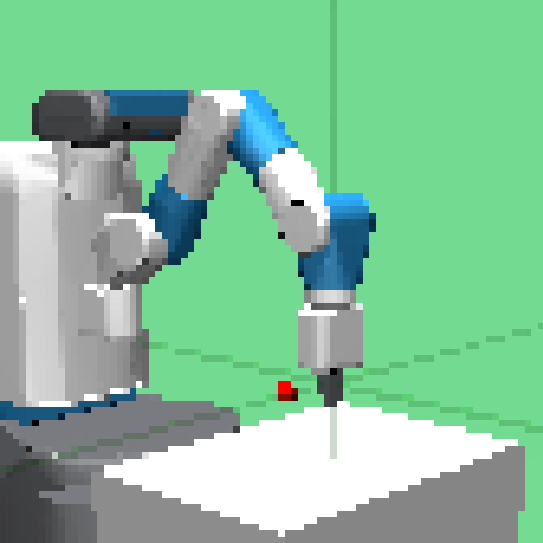
\includegraphics[width=\textwidth]{images/environments/fetch-reach-obs.png}
        \caption{FetchReach}
        \label{fig:envs:reach}
    \end{subfigure}
    \hfill
    \begin{subfigure}[b]{.32\textwidth}
        \centering
        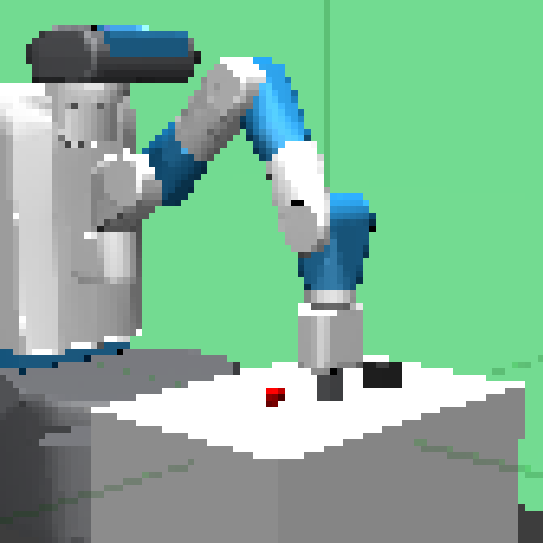
\includegraphics[width=\textwidth]{images/environments/fetch-push-obs.png}
        \caption{FetchPush}
        \label{fig:envs:push}
    \end{subfigure}
    \hfill
    \begin{subfigure}[b]{.32\textwidth}
        \centering
        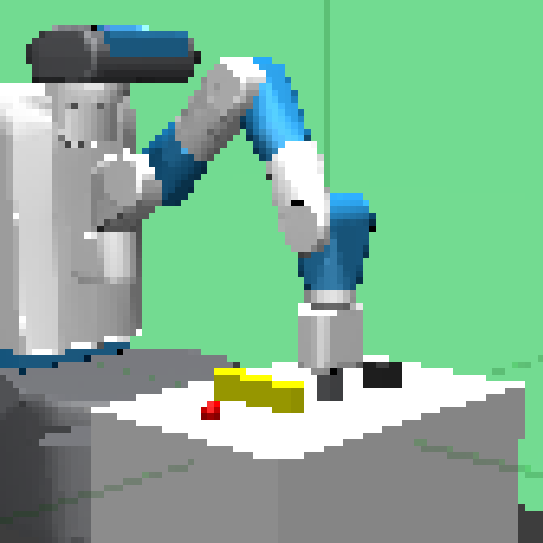
\includegraphics[width=\textwidth]{images/environments/fetch-push-barrier-obs.png}
        \caption{FetchPushBarrier}
        \label{fig:envs:barrier}
    \end{subfigure}
    \caption[Overview of the three environments used in this work.]{Overview of the three environments used in this work. The images show the actual $84\times84$ pixel observations the agents receive. The observations are a cropping of the original image, the gym Fetch environments render. See figure \ref{fig:env-axes} for the original image size.}
    \label{fig:envs-overview}
\end{figure}

\subsection{FetchPushBarrier}
\label{sec:environments:fetch-push-barrier}

The FetchPushBarrier environment is an adaptation of the regular FetchPush environment. The only things changed are the initialization to add a barrier and a cost function.

When initializing the FetchPushBarrier environment, first the gripper and the object are seeded the same as in the FetchPush environment. To position the barrier, first a random position along the x-axis is chosen. See figure \ref{fig:env-axes} for the naming of the axes. The position is drawn to let the barrier extend to the table edges at the most. To sample the placement along the y-axis, first it has to be determined if the barrier should be in front or behind the object, if seen from the camera. If the object is at the very front of the table, the barrier is always placed behind the object. If the object is at the very back, it is placed in front respectively. If the object is in the middle of the table, it is chosen at random if the barrier should be placed in front or behind the object. Afterwards, the exact placement along the y-axis is drawn at random, ensuring a minimum distance to the object, the gripper and the table edge. The size of the barrier is fixed and it is always position parallel to the axes.

After the barrier is placed, the position of the target is drawn at random. The placement is constrained in the y-axis to always be behind the barrier if seen from the object. In the x-axis, the position is constrained to the size of the barrier, to ensure that the object has to be moved around the barrier.

When taking a step in the environment, the reward is calculated just like in the FetchPush environment. For a dense reward, the negative distance between the object and the target is used. The sparse reward is $0$ if the distance between the goal and the target is below a threshold and $-1$ otherwise. Additionally a cost is computed after each step:
\begin{equation}
    C(s,a,s') = \begin{cases}
        0, &\quad\text{if } d \geq 0.1\\
        1-\frac{d}{0.1}, &\quad\text{else}\\
    \end{cases}
\end{equation}
Where $d$ is given by the minimum of the distances of the gripper and object to the barrier.

The maximum steps in the environment is increased to 150, to account for the added difficulty.

\begin{figure}[btp]
    \centering
        \begin{tikzpicture}
            \node at (0,0.3) (image)  {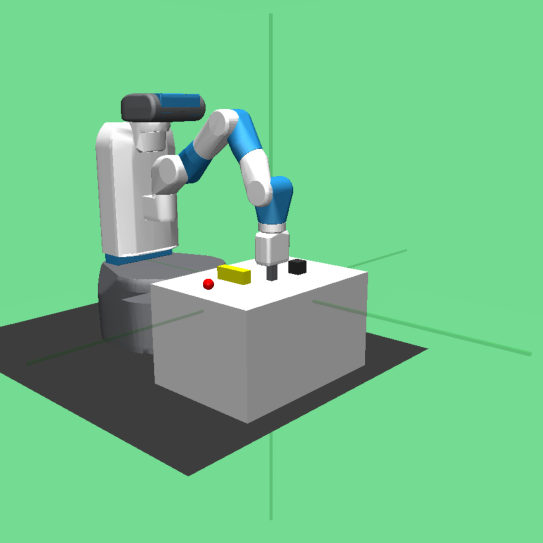
\includegraphics[width=.5\textwidth]{images/environments/fetch-push-barrier.png}};
            \draw[black, thick, ->] (0,0) -- (0,4.2) node[above] {$z$};
            \draw[black, thick, ->] (0,0) -- (4,-1) node[above] {$x$};
            \draw[black, thick, ->] (0,0) -- (4,1.3) node[above] {$y$};
        \end{tikzpicture}
    \caption{Axes in the FetchPushBarrier environment}
    \label{fig:env-axes}
\end{figure}

\section{Experiment Setup}
\label{sec:experiments:setup}

The goal with the experiments was to train an agent using frame stack observations for all three environments described in section \ref{sec:experiments:env}. The experiments use the training setup described in section \ref{sec:algo-high-dim-observations} with an ensemble teacher. This also includes the described option of augmenting the frame stacks with the gripper position to simplify the training. The high dimensional image observations consist of a stack of three frames. Each frame is an image of $84\times84$ colored pixels. 

First, for each environment, an ensemble of three SAC agents using the state was trained. If one of the agents was significantly worse than the others, more agents were trained and the best three picked for the ensemble. See table \ref{tab:ensemble-results} for the exact results of the ensemble agents. Afterwards, the agents using frame stacks or augmented observations are trained with the ensemble. All environments use a dense reward, i.e. a reward is not only given in the case of a success, but at each time step.

The machines used for training either used an Intel Core i9-9900K with 64 GiB of memory and a Nvidia RTX 2080 TI or an AMD Ryzen Threadripper 3960X with 130 GiB of memory and a Nvidia RTX A5000. CUDA version 11.6 was used with both GPUs.

\begin{table}[btp]
	\centering
	\begin{tabular}{lrrrrrr}
\toprule
Environment & Success Rate &     \makecell{Episode\\Reward} &     \makecell{Episode\\Cost} & \makecell{Mean\\Success Rate} & \makecell{Mean\\Reward} & \makecell{Mean\\Cost}\\
\midrule
\multirow{3}*{FetchReach}
 &        1.0 &  -0.600 &          & \multirow{3}*{1.0} & \multirow{3}*{-0.552}\\
 &        1.0 &  -0.572 &          \\
 &        1.0 &  -0.484 &          \\
\midrule
\multirow{3}*{FetchPush}
 &        0.930 &  -3.374 &          & \multirow{3}*{0.901} & \multirow{3}*{-4.134}\\
 &        0.849 &  -4.774 &          \\
 &        0.925 &  -4.253 &          \\
\midrule
\multirow{3}*{FetchPushBarrier}
 &        0.726 & -14.873 & 1.370 & \multirow{3}*{0.761} & \multirow{3}*{-14.083} & \multirow{3}*{1.58}\\
 &        0.790 & -12.439 & 1.075 \\
 &        0.767 & -14.937 & 2.294 \\
\bottomrule
\end{tabular}
	\caption[Overview of the results from all ensembles used in training.]{Overview of the results from all ensembles used in training. All agents were evaluated over 1000 episodes. The same seed was used for all environments.}
	\label{tab:ensemble-results}
\end{table}

\section{Results}
\label{sec:experiments:results}

The following section contains the results of the experiments made during this work. Experiments were made in the environments FetchReach, FetchPush and FetchPushBarrer. The most experiments were made in the FetchReach environment. Training setups that do not perform well in this environment are expected to not have meaningful results in the much harder FetchPush and FetchPushBarrier environments. Therefore some setups were omitted for these environments. The results shown in this section are, if not otherwise stated, averaged over 3 trainings with different random seeds.

\subsection{FetchReach}
\label{sec:results:fetch-reach}

The FetchReach environment is fairly easy and was therefore chosen as a starting point for the experiments in this work. As table \ref{tab:ensemble-results} shows, the three agents of the ensemble for the teacher are all able to solve the task each time. The agents using image observations were trained with regular SAC and SAC together with the two improvements described in section \ref{sec:preliminaries-high-dim-observations}, autoencoders and DrQ. All algorithms were trained with only frame stacks and frame stacks augmented with the gripper position. Additionally, all algorithms were trained with and without the teacher. The $\alpha$ value that defines the importance of the teacher is set to one. This results in a total of 12 combinations. The success rates during training of all 12 setups are plotted in figure \ref{fig:results:reach}. The success rate of SAC state is added as reference. The episode rewards during training are plotted in figure \ref{fig:results:reach-reward}. It does, however, not make sense to compare the rewards of the setups with and without a teacher, since the preference reward algorithm uses reward shaping. Additionally, all agents were evaluated on 1000 episodes. The mean success rate and reward can be seen in table \ref{tab:results:reach}.

The training setups using DrQ were all able to reliably solve the task and they are also the only ones to do so. Adding the gripper information to the observations did, however, increase the sample efficiency. The same is even more true for adding a teacher. Combined, this results in the DrQ agent using augmented states and a teacher almost being as efficient as SAC state. The mean rewards from the evaluation show a similar pattern. The reward is always higher when adding a robot or a teacher. Since the environment uses dense rewards, i.e. the distance between the gripper and the target at each time step, this indicates that the agents are able to solve the task faster.

For the setups using the SAC and SAC-AE algorithms, the picture is not quite as clear. Plain SAC does not benefit from adding the gripper information. Adding a teacher, however, significantly increases the success rate and sample efficiency. SAC-AE benefits from the gripper information and the teacher. Using the teacher results in a higher success rate than adding the gripper information. However, if the gripper information is added to the observations, also adding the teacher does not further increase the success rate. The success rate is actually lower that using SAC-AE with a teacher but without the gripper information. A possible explanation for this lies in the architecture of the SAC-AE agent. The autoencoder only uses the frame stack and tries to reproduce it. It does not benefit from the added gripper information. It also does not benefit from the reward shaping through the teacher, as the autoencoder uses a reconstruction loss and is independent from the reward. This is in contrast to the actor and critic that both benefit from the gripper information and the teacher. This difference could lead to very different updates on the shared CNN encoder during training and could explain the discrepancy in the success rate. The fact that the SAC-AE+robot+teacher setup is outperformed by the same setup without the autoencoder supports this theory.

When looking at the episode reward in figure \ref{fig:results:reach-reward}, it is clear, that DrQ has the highest reward in all setups. This is consistent with the success rate of the DrQ setups. Also, it can be seen that when using a teacher, also adding the gripper information to DrQ increases the sample efficiency.
The episode rewards for the setups using plain SAC and SAC-AE are very similar. Again, this is consistent with the success rates. The success rates of the SAC and SAC-AE setups with a teacher are fairly similar to each other. The same is true for the setups without a teacher.

In general, it can be said that adding a teacher always lead to improvements in the success rate or the sample efficiency over the base version of the algorithm. In fact, for all three algorithms, the best training setup uses a teacher.

\begin{figure}
    \centering
    \begin{subfigure}[b]{.32\textwidth}
        \centering
        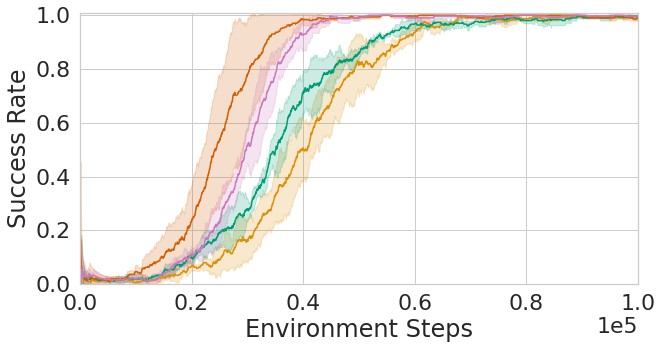
\includegraphics[width=\textwidth]{images/results/reach/drq.png}
        \caption{DrQ}
        \label{fig:results:reach:drq}
    \end{subfigure}
    \hfill
    \begin{subfigure}[b]{.32\textwidth}
        \centering
        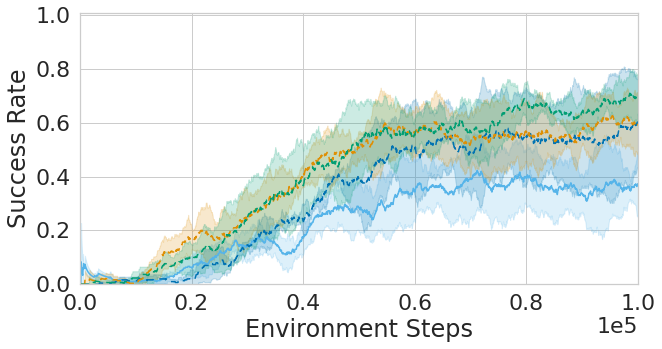
\includegraphics[width=\textwidth]{images/results/reach/sacae.png}
        \caption{SAC-AE}
        \label{fig:results:reach:sacae}
    \end{subfigure}
    \hfill
    \begin{subfigure}[b]{.32\textwidth}
        \centering
        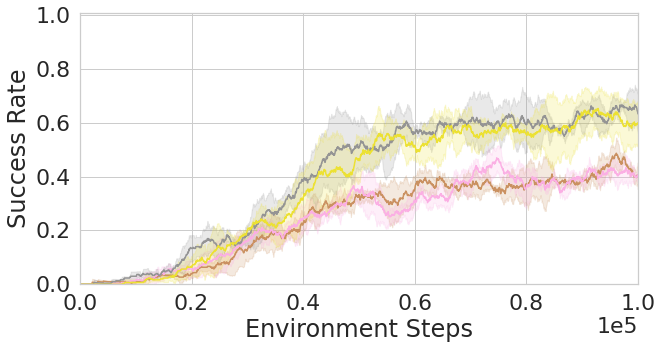
\includegraphics[width=\textwidth]{images/results/reach/sac.png}
        \caption{SAC Pixel}
        \label{fig:results:reach:sac}
    \end{subfigure}
    \hfill
    \begin{subfigure}[b]{.99\textwidth}
        \centering
    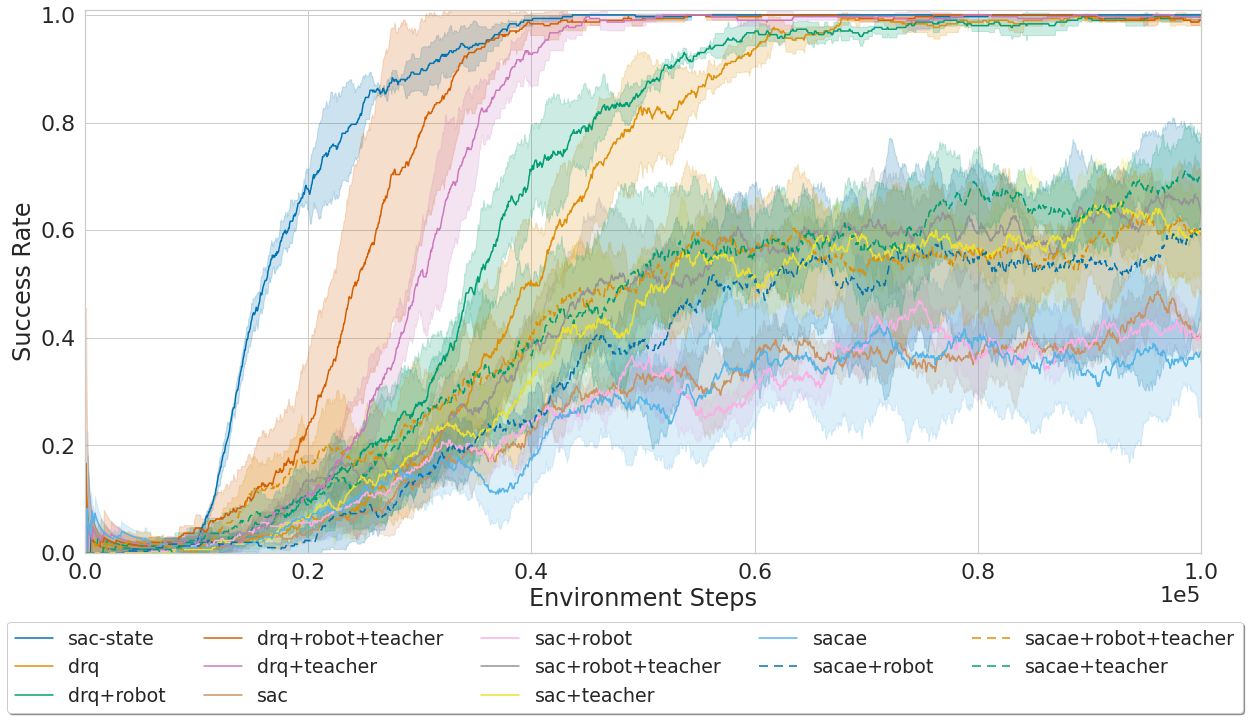
\includegraphics[width=\textwidth]{images/results/reach/all.png}
        \caption{All FetchReach experiments}
        \label{fig:results:reach:all}
    \end{subfigure}
    \caption[The success rates from all experiments on the FetchReach environment.]{The success rates from all experiments on the FetchReach environment. The algorithms SAC pixel, SAC autoencoder and DrQ were each trained with and without augmented states and teachers. As a reference, SAC state is added. The subplots (\subref{fig:results:reach:drq})-(\subref{fig:results:reach:sac}) each show the success rates for one algorithm.}
    \label{fig:results:reach}
\end{figure}

\begin{figure}
    \centering
    \begin{subfigure}[b]{\textwidth}
        \centering
        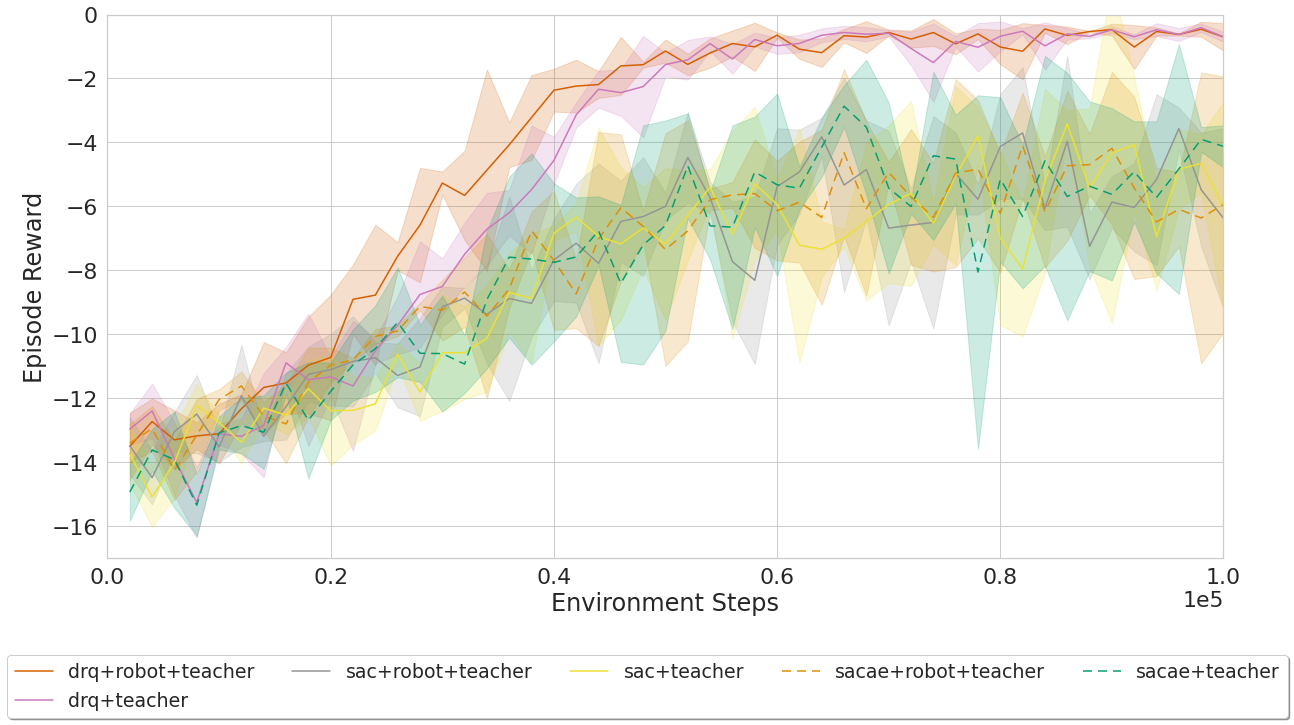
\includegraphics[width=\textwidth]{images/results/reach/reward_teacher.png}
        \caption{Episode reward with a teacher}
        \label{fig:results:reach:reward-teacher}
    \end{subfigure}
    \hfill
    \begin{subfigure}[b]{\textwidth}
        \centering
        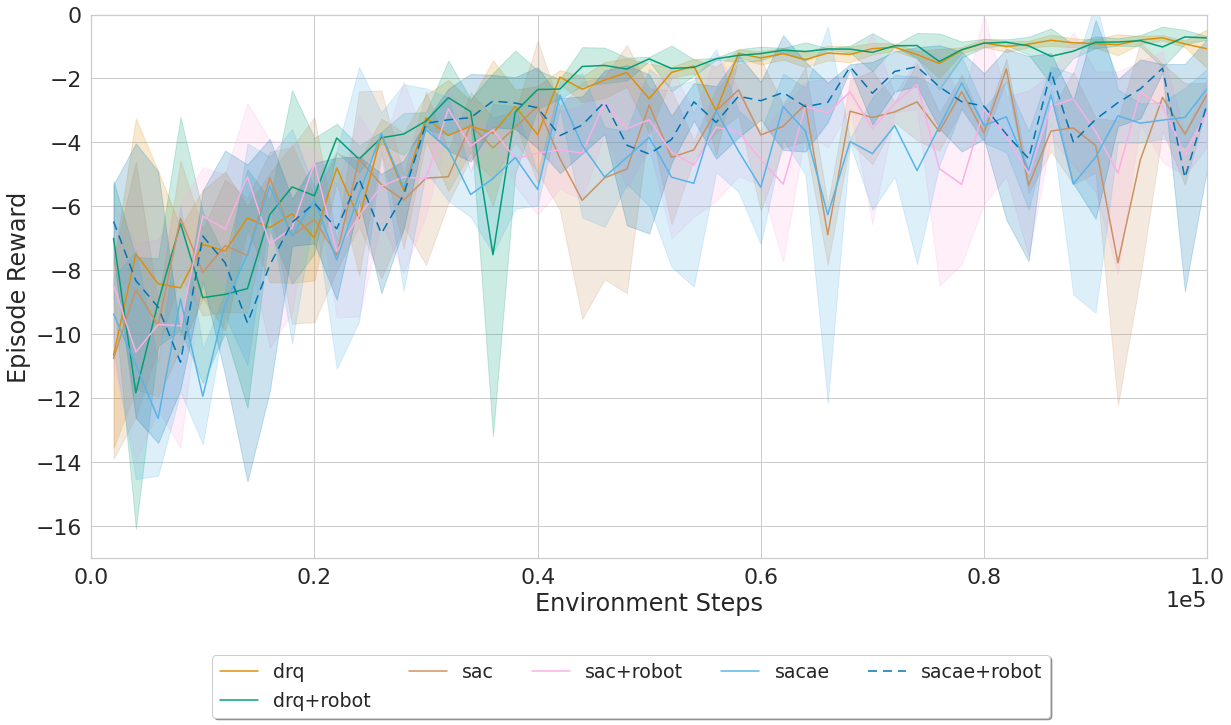
\includegraphics[width=\textwidth]{images/results/reach/reward_no_teacher.png}
        \caption{Episode reward without a teacher}
        \label{fig:results:reach:reward_no_teacher}
    \end{subfigure}
    \caption[The episode rewards from all experiments on the FetchReach environment.]{The episode rewards from all experiments on the FetchReach environment. The algorithms SAC pixel, SAC autoencoder and DrQ were each trained with and without augmented states and teachers. Since the preference reward algorithm uses reward shaping, it does not make sense to compare the experiments with and without a teacher.}
    \label{fig:results:reach-reward}
\end{figure}

\begin{table}[btp]
    \centering
    \begin{tabular}{lllrr}
\toprule
Algorithm & Robot & Teacher & Mean Success Rate & Mean Episode Reward \\
\midrule
\multirow{4}{*}{drq} & \multirow{2}{*}{False} & False &             0.994 &      -0.852 \\
      &      & True &             0.994 &      -0.720 \\
\cline{2-5}
      & \multirow{2}{*}{True} & False &             0.993 &      -0.763 \\
      &      & True &             0.996 &      -0.698 \\
\cline{1-5}
\cline{2-5}
\multirow{4}{*}{sac} & \multirow{2}{*}{False} & False &             0.425 &      -3.360 \\
      &      & True &             0.608 &      -2.945 \\
\cline{2-5}
      & \multirow{2}{*}{True} & False &             0.393 &      -3.622 \\
      &      & True &             0.628 &      -2.912 \\
\cline{1-5}
\cline{2-5}
\multirow{4}{*}{sacae} & \multirow{2}{*}{False} & False &             0.388 &      -3.484 \\
      &      & True &             0.657 &      -2.787 \\
\cline{2-5}
      & \multirow{2}{*}{True} & False &             0.573 &      -2.882 \\
      &      & True &             0.588 &      -3.084 \\
\bottomrule
\end{tabular}
    \caption[Mean success rate and reward for all agents trained on the FetchReach environment.]{Mean success rate and reward for all agents trained on the FetchReach environment. The shown values are the mean over the three agents trained for each setup. All agents were evaluated on 1000 episodes. The environments were initialized with the same seed. The preference reward algorithm is not used during evaluation. Therefore, the reward shown here is the environment reward.}
    \label{tab:results:reach}
\end{table}

\subsection{FetchPush}
\label{sec:results:fetch-push}

Only agents trained with DrQ were able to reliably solve the FetchReach environment. Since the FetchPush environment is significantly harder than the FetchReach environment, all agents were trained with DrQ. Additionally, the robot state augmentations were used for all experiments. Again, this is based on the experience with FetchReach, where this improved the sample efficiency.

Experiments were conducted with and without a teacher. When a teacher was used, the fixed $\alpha$ values of $1.0$ and $0.5$ were tried. Additionally, an adaptive $\alpha$ was used as described in section \ref{sec:adaptive-alpha}. The adaptive $\alpha$ is based on the environment reward. To stabilize the adaptive $\alpha$ value, it is calculated from a moving average of the environment reward for one episode with a coefficient of $0.01$. The $\alpha$ value was then given by the following function:
\[
\alpha(r_{env}) = \begin{cases}
        1, &\quad\text{if } r_{env} < -20\\
        1-\frac{-20-r_{env}}{-20}, &\quad\text{else}\\
    \end{cases}
\]
With this function, the $\alpha$ value starts at one at the beginning of the training and gets lower once the agent surpasses an environment reward of $-20$ per episode. At a non achievable environment reward of zero, the $\alpha$ value would also reach zero.

Figure \ref{fig:results:push-success} shows the success rates during training of all experiments. The different $\alpha$ values of the experiments with a teacher and their development during training are plotted in figure \ref{fig:results:push-alpha}. The rewards during training are not shown here, as all experiments use different $\alpha$ values and the rewards are therefore not comparable. All trained agents were evaluated on 1000 episodes. The mean success rates and episode rewards can be seen in table \ref{tab:results:push}.

When looking at the success rate of the experiment without a teacher, it is clearly visible that there is no noticeable training effect. The success rate does not change over the course of the training. The way the FetchPush environment is initialized, it is possible for the object and the target to touch each other from the beginning. The environment is therefore sometimes solved without the robot moving the object. Most likely this is why the success rate is not zero when training without the teacher.

When training with a fixed $\alpha$ of one, the agents were able to solve the task in roughly $40\%$ of the cases during training. When evaluated over 1000 episodes, the mean success rate was $40.3\%$. The success rate of the agents trained with an $\alpha$ of $0.5$ increased a little slower that the one with an $\alpha$ of one, but surpassed it at some point. During training, a success rate of up to $70\%$ was reached. However, the success rate shows some fluctuation. In the final evaluation, the success rate was $61.5\%$. During training, the success rate is calculated based on the last 100 episodes. The final evaluation is calculated using 1000 episodes. This explains the difference in the results. A possible explanation for the higher success rate with a lower $\alpha$ lies in the quality of the teacher. As it can be seen in table \ref{tab:ensemble-results}, the ensemble, the teacher consists of, has a mean success rate of $90.1\%$. With an $\alpha$ of one, the agent in training can only learn to imitate the teacher. If, however, the teacher is not acting perfectly, the agent will learn subpar actions. With a lower $\alpha$ value, the agent gets direct feedback from the environment an can also learn from this.

With the adaptive $\alpha$ we saw a success rate very similar to the experiments with a fixed $\alpha$ of 0.5. Figure \ref{fig:results:push-alpha} shows the development of the $\alpha$ value over the course of the training. The adaptive value dropped significantly below the fixed value of 0.5. However, this did not lead to changes in the success rate. In the final evaluation, we see a slight improvement of the agents with an adaptive $\alpha$ over the ones with a fixed $\alpha$ of 0.5, with regards to both the success rate and the mean episode reward.

One problem that might lower the performance with the adaptive $\alpha$ lies in the architecture of Off-policy RL algorithms in combination with the preference reward algorithm. While both the environment reward $r_{env}$ and the teacher reward $r_{teacher}$ are in range $[0,1]$, it is possible that $r_{teacher}$ is significantly higher than $r_{env}$. This can happen especially if $r_{env}$ is very small for each step. When $r_{env}$ increases and the $\alpha$ is reduced, this can lead to overall lower values of the preference reward $r_{pr}$, although the agent is performing better. Since the replay buffer only stores $r_{pr}$, the agent then learns the wrong behavior. A possible solution for this would be to store both $r_{env}$ and $r_{teacher}$ and only calculate $r_{pr}$ when it is needed for the training, using the current $\alpha$ value. However, this possible improvement was left for future works, due to time restricitions.

Overall, the adaptive $\alpha$ slightly improved the performance. However, the main benefit is that it gives us a different way to set the importance of the teacher. It can be hard to set a good $\alpha$ value. With the adaptive $\alpha$, we instead have to set a reward threshold when to start lowering the $\alpha$ value. Note that this is only one possibility to adapt the $\alpha$ value. Other functions may be used as well.

\begin{figure}
    \centering
    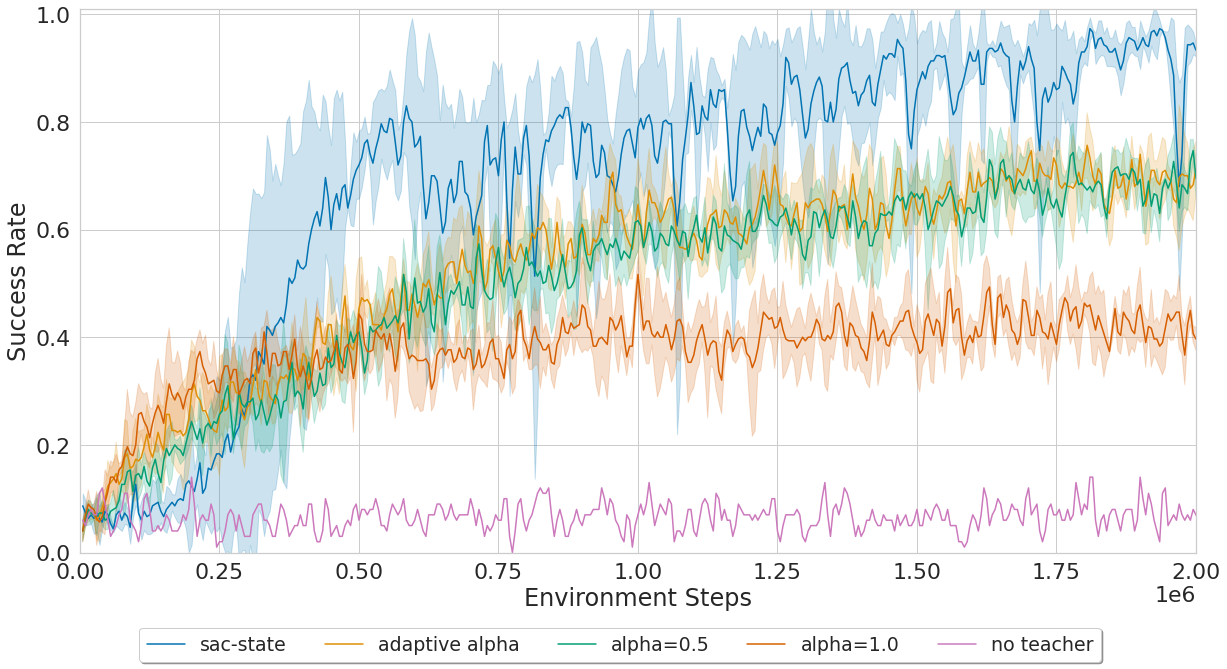
\includegraphics[width=\textwidth]{images/results/push/success_rate.png}
    \caption[The success rates from all experiments on the FetchPush environment.]{The success rates from all experiments on the FetchPush environment. All agents were trained with DrQ and the robot state augmentations. As a reference, SAC state is added. In contrast to the other experiments, the agent without a teacher was only trained with one seed. It is however clearly visible that there is no noticeable training effect.}
    \label{fig:results:push-success}
\end{figure}
\begin{figure}
    \centering
    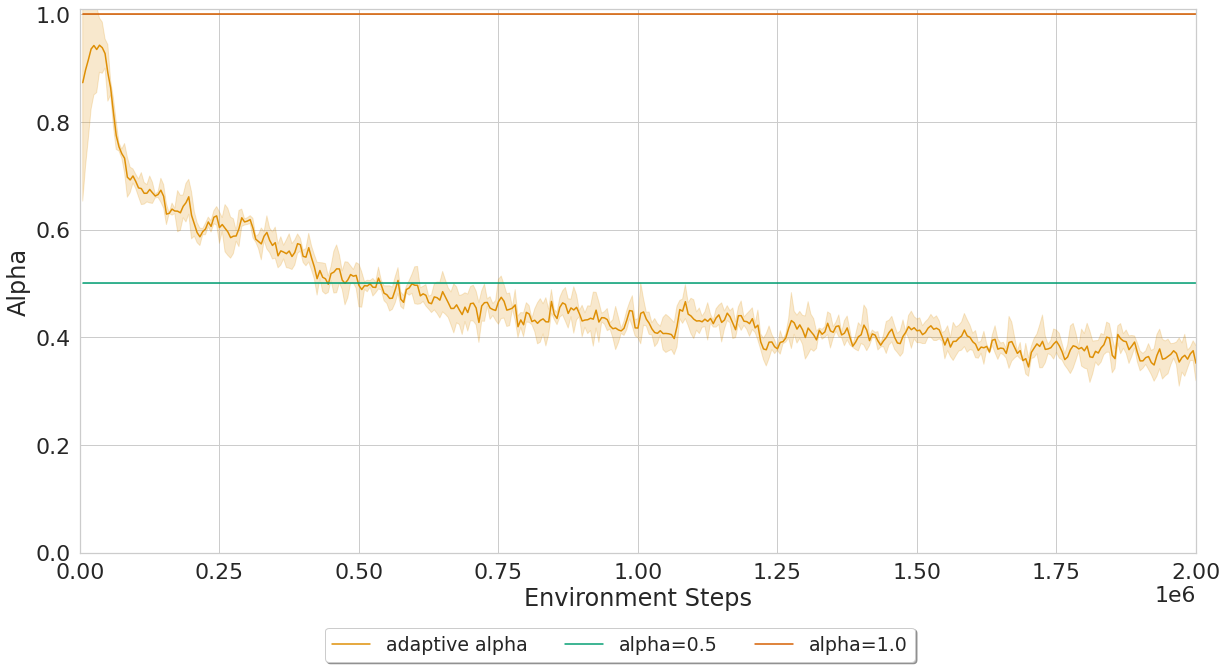
\includegraphics[width=\textwidth]{images/results/push/alpha.png}
    \caption[The $\alpha$ value from all experiments on the FetchPush environment.]{The $\alpha$ value from all experiments on the FetchPush environment. The $\alpha$ value of the experiments with an adaptive $\alpha$ is calculated with a function based on the environment reward. See section \ref{sec:adaptive-alpha} for reference.}
    \label{fig:results:push-alpha}
\end{figure}

\begin{table}[btp]
    \centering
    \begin{tabular}{lrr}
\toprule
Experiment & Mean Success Rate & Mean Episode Reward \\
\midrule
Adaptive $\alpha$ &             0.617 &              -7.641 \\
$\alpha$=0.5      &             0.615 &              -8.338 \\
$\alpha$=1.0      &             0.403 &             -11.269 \\
No teacher     &             0.071 &             -17.316 \\
\bottomrule
\end{tabular}


    \caption[Mean success rate and reward for all agents trained on the FetchPush environment.]{Mean success rate and reward for all agents trained on the FetchPush environment. The shown values are the mean over the three agents trained for each setup. All agents were evaluated on 1000 episodes. The environments were initialized with the same seed. The preference reward algorithm is not used during evaluation. Therefore, the reward shown here is the environment reward.}
    \label{tab:results:push}
\end{table}

\subsection{FetchPushBarrier State}
\label{sec:results:fetch-push-barrier-state}

As described in section \ref{sec:environments:fetch-push-barrier}, the FetchPushBarrier environment is an adaptation from the FetchPush environment that adds a cost function. To represent the cost, the three methods from section \ref{sec:safety}, reward based, safety training, and safety evaluation, were used. The parameters $\lambda_r$ and $\lambda_c$ that define the importance of the reward and the cost in the reward based approach were both set to one. All agents were trained using the state space as observations. 

Figure \ref{fig:results:barrier-state-success} shows the success rate and figure \ref{fig:results:barrier-state-cost} the cost during training. To show the effect of the safety evaluation, the agents were evaluated every 25000 training steps. The figures \ref{fig:results:barrier-state-cost-train} and \ref{fig:results:barrier-state-cost-eval} show the cost during training and periodic evaluation respectively. For the periodic evaluation, the safety evaluation was used with the parameter $n=10$ and $\delta=0.05$. The parameter $n$ defines how many actions are sampled from the policy for each action that is needed from the agent. The parameter $\delta$ defines the threshold when to select the action that is expected to maximize the reward or minimizes the cost. Additionally, all agents were evaluated on 1000 episodes. The results are shown in table \ref{tab:results:barrier-state}. The values are averaged over the three agents trained with each algorithm.

When looking at the success rate, all algorithms show a similar sample efficiency. However, the safety training shows a higher success rate than the reward based approach. The safety evaluation performed worse than the reward based approach. In the final evaluation, the safety training and the reward based approach have very similar success rates of $68\%$ and $67.5\%$.

The cost during training, as plotted in figure \ref{fig:results:barrier-state-cost-train} shows a similar picture. Again, the safety training performs the best, followed by the reward based approach. The high cost from the safety evaluation was expected, as only the reward is optimized during training with the safety evaluation. In the final evaluation, the safety training clearly outperforms the reward based approach with a mean cost of $1.757$ against $3.115$. With the safety training there is also a clearly visible training effect with regards to the cost. The cost gets lower, the further the training progressed. With the reward based approach, the training effect is not quite as visible. This might be due to the fact that the final cost is not as good. When looking at the cost during the periodic evaluation, the safety evaluation clearly lowered the costs, but is still significantly worse than the two other approaches. Also the cost seem to be very similar over the course of the training after a short period with lower costs. This could be explained with the way the FetchPushBarrier  environment works. To produce costs, the agent first needs to learn to move the object towards the target, since the barrier is always located between the object and the target. As the agent improves, it will more often come into states were costs are possible, mitigating the effect of the improved avoidance of costs.

\begin{figure}
    \centering
    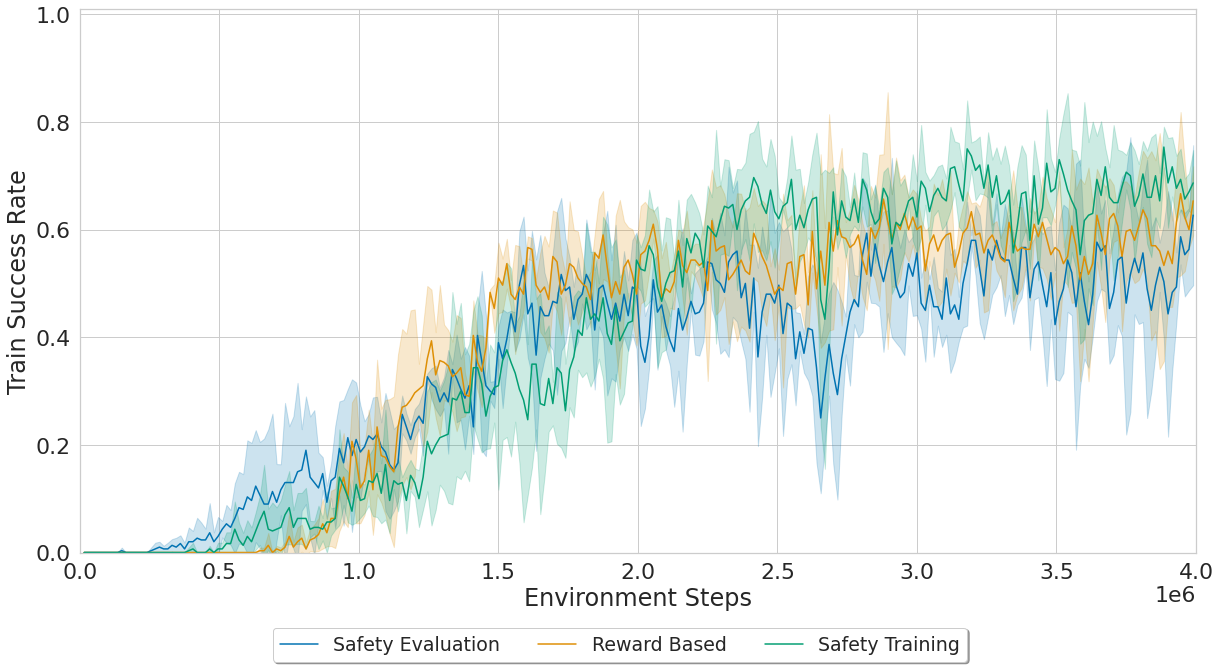
\includegraphics[width=\textwidth]{images/results/push-barrier-state/success.png}
    \caption[The success rates from on the FetchPushBarrier state experiments.]{The success rates from the FetchPushBarrier state experiments. The FetchPushBarrier environment was trained with the reward based approach as well as the safety training and safety evaluation algorithm.}
    \label{fig:results:barrier-state-success}
\end{figure}

\begin{figure}
    \centering
    \begin{subfigure}[b]{\textwidth}
        \centering
        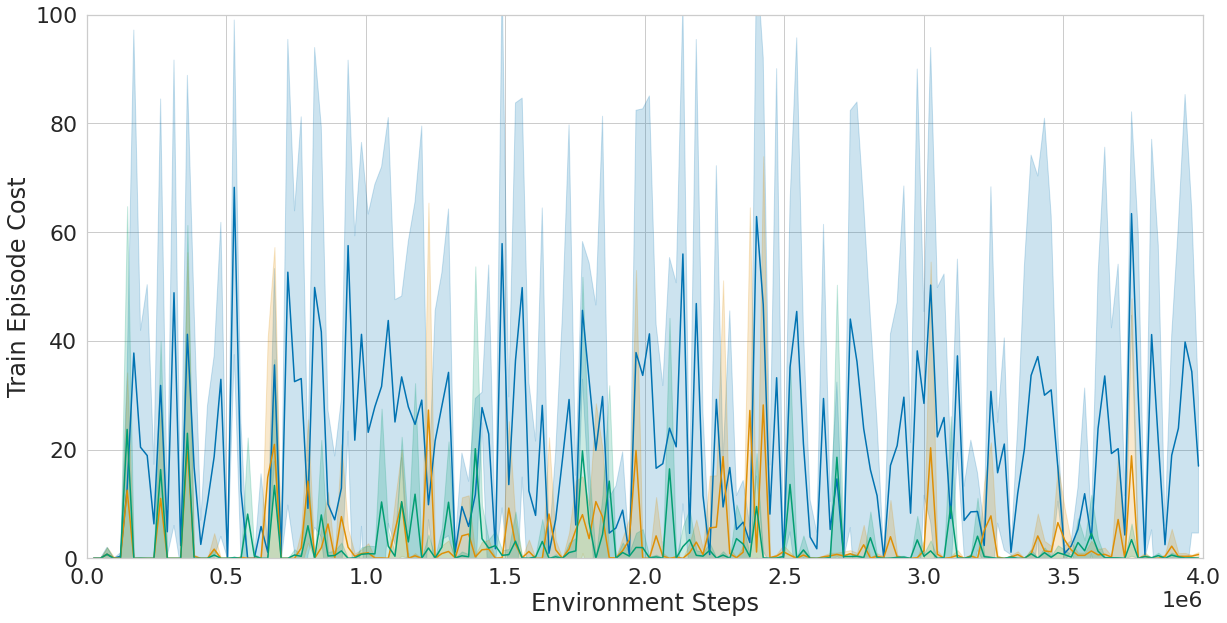
\includegraphics[width=\textwidth]{images/results/push-barrier-state/cost.png}
        \caption{Episode cost during training}
        \label{fig:results:barrier-state-cost-train}
    \end{subfigure}
    \hfill
    \begin{subfigure}[b]{\textwidth}
        \centering
        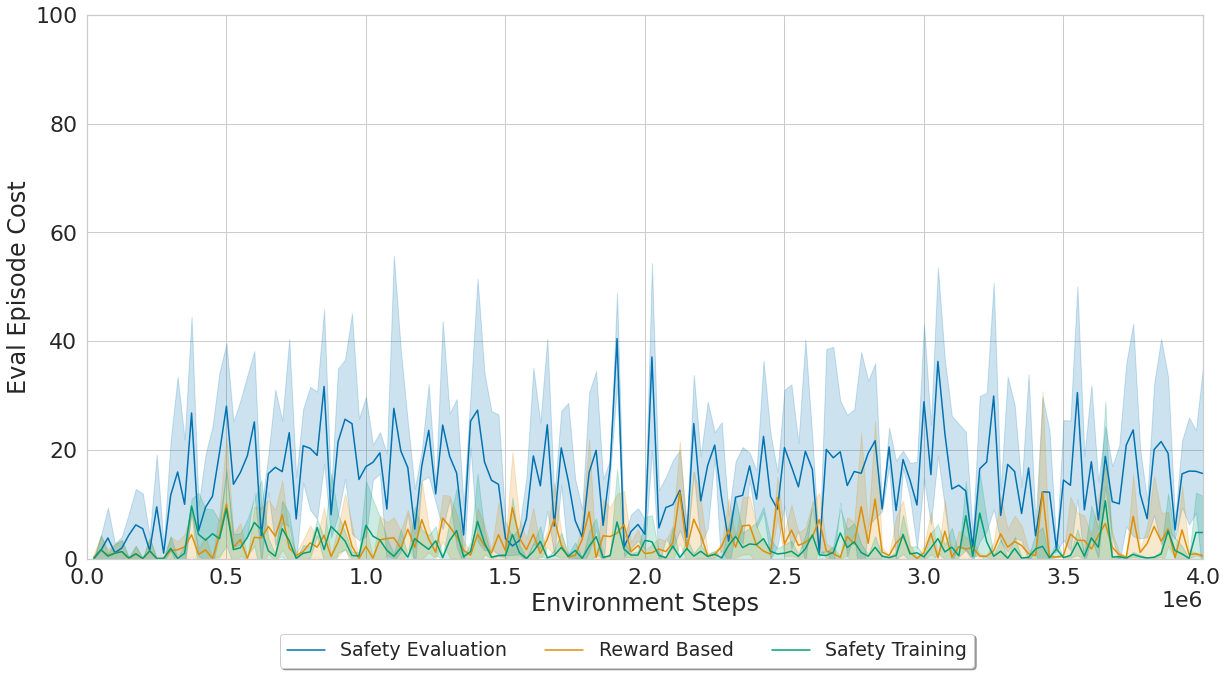
\includegraphics[width=\textwidth]{images/results/push-barrier-state/eval_cost.png}
        \caption{Episode cost from periodic evaluation during training}
        \label{fig:results:barrier-state-cost-eval}
    \end{subfigure}
    \caption[The episode cost from the FetchPushBarrier state experiments.]{The episode cost from the FetchPushBarrier state experiments. The FetchPushBarrier environment was trained with the reward based approach as well as the safety training and safety evaluation algorithm. During the training, the agents were periodically evaluated. Subplot (\subref{fig:results:barrier-state-cost-train}) shows the costs during training and subplot (\subref{fig:results:barrier-state-cost-eval}) the cost during the evaluation. The safety evaluation used the parameters $n=10$ and $\delta=0.05$.}
    \label{fig:results:barrier-state-cost}
\end{figure}

\begin{table}[btp]
    \centering
    \begin{tabular}{lrrr}
\toprule
Algorithm & Mean Success Rate & Mean Reward & Mean Cost \\
\midrule
Reward Based      &             0.675 &     -16.466 &     3.115 \\
Safety Evaluation deactivated      &             0.551 &     -15.710 &    21.057 \\
Safety Evaluation activated &             0.576 &     -15.498 &    16.069 \\
Safety Training   &             0.680 &     -13.278 &     1.757 \\
\bottomrule
\end{tabular}
    \caption[Mean success rate, reward and cost for all agents trained on the FetchPushBarrier environment using state.]{Mean success rate and reward for all agents trained on the FetchPushBarrier environment using state. The shown values are the mean over the three agents trained for each setup. All agents were evaluated on 1000 episodes. The safety evaluation agents were evaluated with the parameters $n=10$ and $\delta=0.05$. This choice of parameters resulted in the lowest mean episode cost with the safety evaluation.}
    \label{tab:results:barrier-state}
\end{table}

The three agents trained for the safety evaluation were additionally evaluated with different values for $n$ and $\delta$. For $n$, the values 1, 2, 5, and 10 were used. For $\delta$ the values 0.05, 0.1, 0.2, and 0.5. Not that for $n=1$ the choice of $\delta$ does not matter. Each agent was evaluated for 1000 episodes with each parameter combination. Table \ref{tab:results:barrier-state-safety-eval} shows the mean success rate, episode reward and episode cost for each parameter combination. The mean is calculated over the results from the three agents. Additionally, the results are visualized in figure \ref{fig:results:barrier-state-safety-eval}.

It is clearly visible that a higher value for $n$ results in a lower cost. This is easily explained with the way the algorithm works. The algorithm samples $n$ actions from the actor. With a higher value for $n$, the probability to get a low cost action is higher. However, a higher value also results in a longer execution time. Therefore, the parameter $n$ has to be chosen with a trade-off between cost and execution time. Drawing more sample also slightly increased the success rate. This can be explained by the stochastic nature of the actors. The more actions are drawn the higher the probability to get a good action. However, since the action with the lowest expected cost is selected, the effect on the success rate is only marginal. When looking at the mean episode reward, the difference between the experiments is so little that an interpretation makes no sense.

The value for $\delta$ seems to make no difference in all of the experiments. This is explained by a misconception when designing this evaluation. The choices for $\delta$ are within the range of the cost of one action, while the safety critic learns the expected cost for a whole episode. Therefore, the expected cost is always higher than $\delta$ and the action with the lowest expected cost is selected.

Overall, it can be said that the safety evaluation was able to reduce the cost, with a trade-off between the cost and the execution time. However, the cost is still a lot higher than the cost produced by an agent trained with the safety training algorithm or the reward based approach.

\begin{figure}
    \centering
    \begin{subfigure}[b]{.49\textwidth}
    \centering
    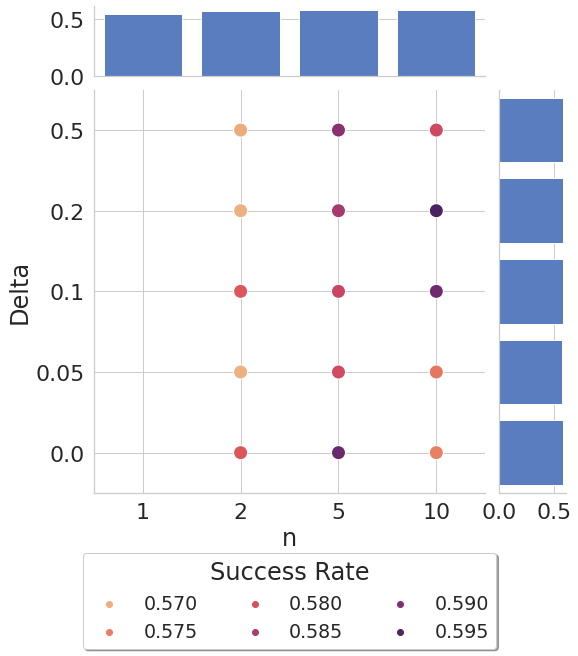
\includegraphics[width=\textwidth]{images/results/push-barrier-state/safety_eval_success.png}
    \caption{Safety evaluation success rate}
    \label{fig:results:barrier-state-safety-eval-success}
    \end{subfigure}
    \hfill
    \begin{subfigure}[b]{.49\textwidth}
    \centering
    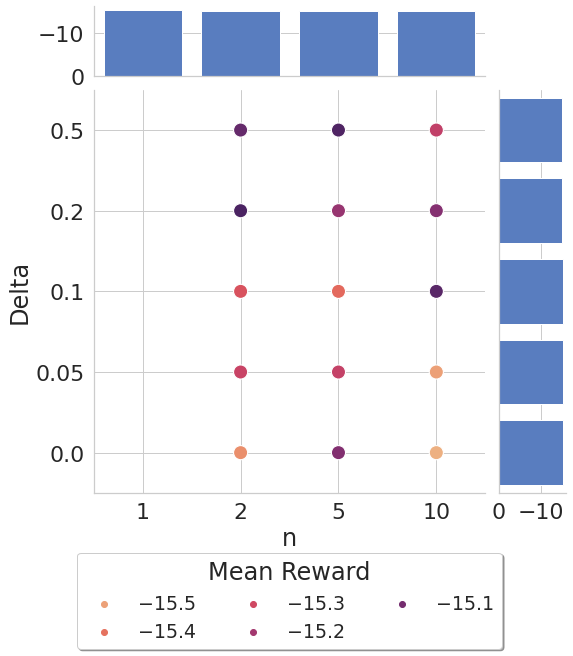
\includegraphics[width=\textwidth]{images/results/push-barrier-state/safety_eval_reward.png}
    \caption{Safety evaluation reward}
    \label{fig:results:barrier-state-safety-eval-reward}
    \end{subfigure}
    \hfill
    \begin{subfigure}[b]{.6\textwidth}
    \centering
    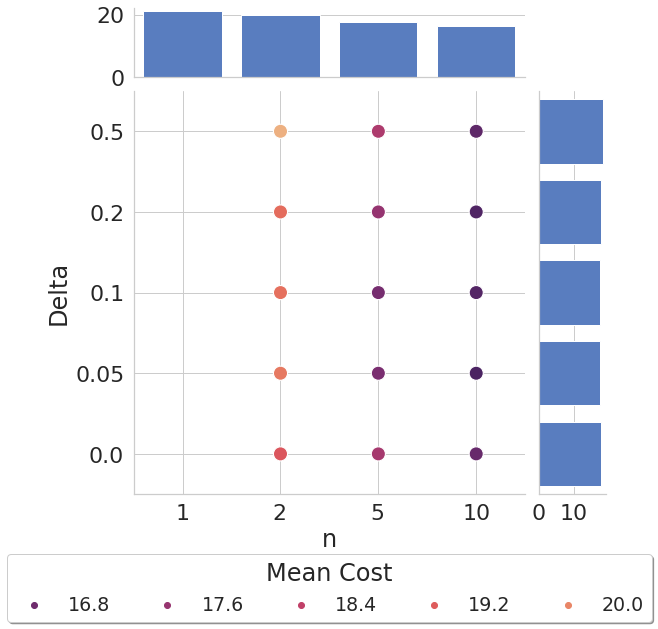
\includegraphics[width=\textwidth]{images/results/push-barrier-state/safety_eval_cost.png}
    \caption{Safety evaluation reward}
    \label{fig:results:barrier-state-safety-eval-cost}
    \end{subfigure}
    \caption[Analysis of the safety evaluation algorithm.]{Analysis of the safety evaluation algorithm with different values for $n$ and $\delta$. The three agents trained for safety evaluation were each evaluated with the different parameters. For $n=1$ the value of $\delta$ makes no difference. The subplots (\subref{fig:results:barrier-state-safety-eval-success})-(\subref{fig:results:barrier-state-safety-eval-cost}) show the success rate, mean reward and mean cost for all parameter combinations. The bar plots on the side show the mean values for the specific values for $n$ or $\delta$, averaged over the other parameter.}
    \label{fig:results:barrier-state-safety-eval}
\end{figure}

\begin{table}[btp]
    \centering
    \begin{tabular}{llrrr}
\toprule
n & $\delta$ & \makecell{Mean\\Success Rate} & \makecell{Mean\\Episode Reward} & \makecell{Mean\\Episode Cost} \\
\midrule
1  &   -  &             0.550 &     -15.608 &    21.177 \\
\cline{1-5}
\multirow{5}{*}{2} & 0.00 &             0.579 &     -15.460 &    19.089 \\
   & 0.05 &             0.570 &     -15.280 &    19.756 \\
   & 0.10 &             0.579 &     -15.329 &    19.588 \\
   & 0.20 &             0.570 &     -15.004 &    19.510 \\
   & 0.50 &             0.570 &     -15.065 &    20.797 \\
\cline{1-5}
\multirow{5}{*}{5} & 0.00 &             0.592 &     -15.125 &    17.886 \\
   & 0.05 &             0.581 &     -15.273 &    17.024 \\
   & 0.10 &             0.582 &     -15.382 &    16.939 \\
   & 0.20 &             0.586 &     -15.174 &    17.564 \\
   & 0.50 &             0.589 &     -15.014 &    18.023 \\
\cline{1-5}
\multirow{5}{*}{10} & 0.00 &             0.575 &     -15.531 &    16.647 \\
   & 0.05 &             0.576 &     -15.498 &    16.069 \\
   & 0.10 &             0.592 &     -15.038 &    16.259 \\
   & 0.20 &             0.596 &     -15.132 &    16.198 \\
   & 0.50 &             0.581 &     -15.264 &    16.464 \\
\bottomrule
\end{tabular}


    \caption[Analysis of the safety evaluation algorithm.]{Analysis of the safety evaluation algorithm with different values for $n$ and $\delta$. The three agents trained for safety evaluation were each evaluated with the different parameters. For $n=1$ the value of $\delta$ makes no difference. The values shown here are the mean of the three agents.}
    \label{tab:results:barrier-state-safety-eval}
\end{table}

\subsection{FetchPushBarrier Pixel}
\label{sec:results:fetch-push-barrier-pixel}

\begin{table}[btp]
    \centering
    \begin{tabular}{llrrr}
\toprule
Algorithm & $\alpha$   & \makecell{Mean\\Success Rate} & \makecell{Mean\\Episode Reward} & \makecell{Mean\\Episode Cost} \\
\midrule
\multirow{2}{*}{Reward Based} & 0.5 &             0.003 &     -45.532 &     2.425 \\
                & 1.0 &             0.003 &     -52.985 &     6.809 \\
\cline{1-5}
\multirow{2}{*}{Safety Training} & 0.5 &             0.003 &     -40.041 &     3.080 \\
                & 1.0 &             0.001 &     -46.977 &     2.220 \\
\bottomrule
\end{tabular}
    \caption[Mean success rate, reward and cost for all agents trained on the FetchPushBarrier environment using pixels.]{Mean success rate and reward for all agents trained on the FetchPushBarrier environment using pixels. For each setup only one agent was trained. All agents were evaluated on 1000 episodes.}
    \label{tab:results:barrier-drq}
\end{table}

The final experiment was conducted on the FetchPushBarrier environment using image observations. It uses the combination of the preference reward algorithm and a cost representation. Experiments were conducted with the reward based approach and the safety training, as these had the highest success rates in the previous experiments. When using the reward based approach, first the reward and cost are combined and then the preference reward is calculated. Unlike in definition \ref{def:preference-reward}\ref{enm:pr:external-reward}, the environment reward $r_{env}$ is not given by the MDPs reward function, but by the combination of the reward and the cost function $R_{cost}(s,a,s')$. See equation \ref{eq:reward-based-cost} for the definition of the function. The combined reward function is then given by:
\[
r_{pr} = \alpha * r_{teacher} + (1-\alpha) * \big(\lambda_r R(s,a,s') - \lambda_c C(s,a,s')\big)
\]
Again, the parameters $\lambda_r$ and $\lambda_c$ for the reward based approach were both set to one. We trained agents using $\alpha$ values of $0.5$ and one. The parameter $\alpha$ defines the importance of the teacher in contrast to the environment reward.

After the training, we evaluated the agents on 1000 episodes. The results are shown in table \ref{tab:results:barrier-drq}. None of the agents was able to reach a meaningful success rate. However, all of the agents where able to solve the task at least once. In contrast to the FetchPush environment, the FetchPushBarrier environment is always initialized in a way that requires the agent to move the object to solve the task. This indicates that the agents did learn some behavior required to solve the task but not quite how to solve it. This theory is supported when looking at videos from the evaluation. Figure \ref{fig:results:barrier-drq-frames} shows 5 frames from a video recorded during the evaluation of the agent trained with safety training and an $\alpha$ of $0.5$. The agent learned to move the object around the barrier and towards the target, but does not move it quite far enough. The episode is therefore not considered a success.

For the sake of completeness, figure \ref{fig:results:barrier-drq-cost} shows the development of the cost during the training. However, since the goal for the agents is to solve the task while keeping the cost low, it makes little sense to interpret the cost if the task is not solved. An agent that does not move the object and always keeps a distance to the barrier could achieve minimal cost, but would never solve the task. Because there is little to interpret with regards to the result for this experiment, we only trained one agent for each parameter combination.

We see two reasons why we were not able to reliably solve the FetchPushBarrier environment using high dimensional image observations. The first reasons is the difficulty of the environment itself. Even when training on state observations, our agents where only able to reach a mean success rate of $68\%$. The second reason is connected to the first. The teacher we used is an ensemble of SAC state agents. We trained six agents in total using SAC state and selected the three best agents. By doing so, we were able to increase the mean success rate of the teacher to $76.1\%$. This can be seen in table \ref{tab:ensemble-results}. However, this is significantly worse than the teacher for FetchReach and FetchPush. Figure \ref{fig:results:barrier-drq-ensemble-bar} shows the success rates in relation to each other. Additionally, it shows the mean confidence of the teachers. To calculate the mean confidence, first the best agent of each ensemble, with regards to the success rate, was selected. This agent was evaluated on 1000 episodes. For each action, the confidence was calculated using all three agents. The mean of the confidence of all actions is shown in the chart. The teacher for the FetchPushBarrier environment also has the lowest mean confidence. This means that the agents of the ensemble propose different actions as the best action. However, this makes it hard for the student to learn the best action. The most drastic example would be, if two of the teacher agents want to pass the barrier on different sides. It is up to future work to show if an improved teacher can lead to better performance on the FetchPushBarrier environment using high dimensional image observations.

\begin{figure}
    \centering
    \begin{subfigure}[b]{.19\textwidth}
    \centering
    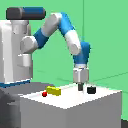
\includegraphics[width=\textwidth]{images/results/push-barrier-drq/frames/frame_0.png}
    \end{subfigure}
    \begin{subfigure}[b]{.19\textwidth}
    \centering
    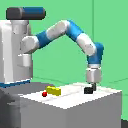
\includegraphics[width=\textwidth]{images/results/push-barrier-drq/frames/frame_1.png}
    \end{subfigure}
    \begin{subfigure}[b]{.19\textwidth}
    \centering
    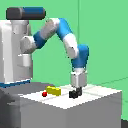
\includegraphics[width=\textwidth]{images/results/push-barrier-drq/frames/frame_2.png}
    \end{subfigure}
    \begin{subfigure}[b]{.19\textwidth}
    \centering
    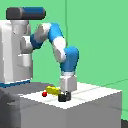
\includegraphics[width=\textwidth]{images/results/push-barrier-drq/frames/frame_3.png}
    \end{subfigure}
    \begin{subfigure}[b]{.19\textwidth}
    \centering
    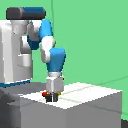
\includegraphics[width=\textwidth]{images/results/push-barrier-drq/frames/frame_4.png}
    \end{subfigure}
    \hfill
    \caption[Frames from a video recorded on the FetchPushBarrier - Pixel environment]{Frames from a video recorded on the FetchPushBarrier - Pixel environment. The video was recorded with the agent trained using safety training and an $\alpha$ of $0.5$. Between each image, 5 frames where skipped.}
    \label{fig:results:barrier-drq-frames}
\end{figure}

\begin{figure}[btp]
    \centering
    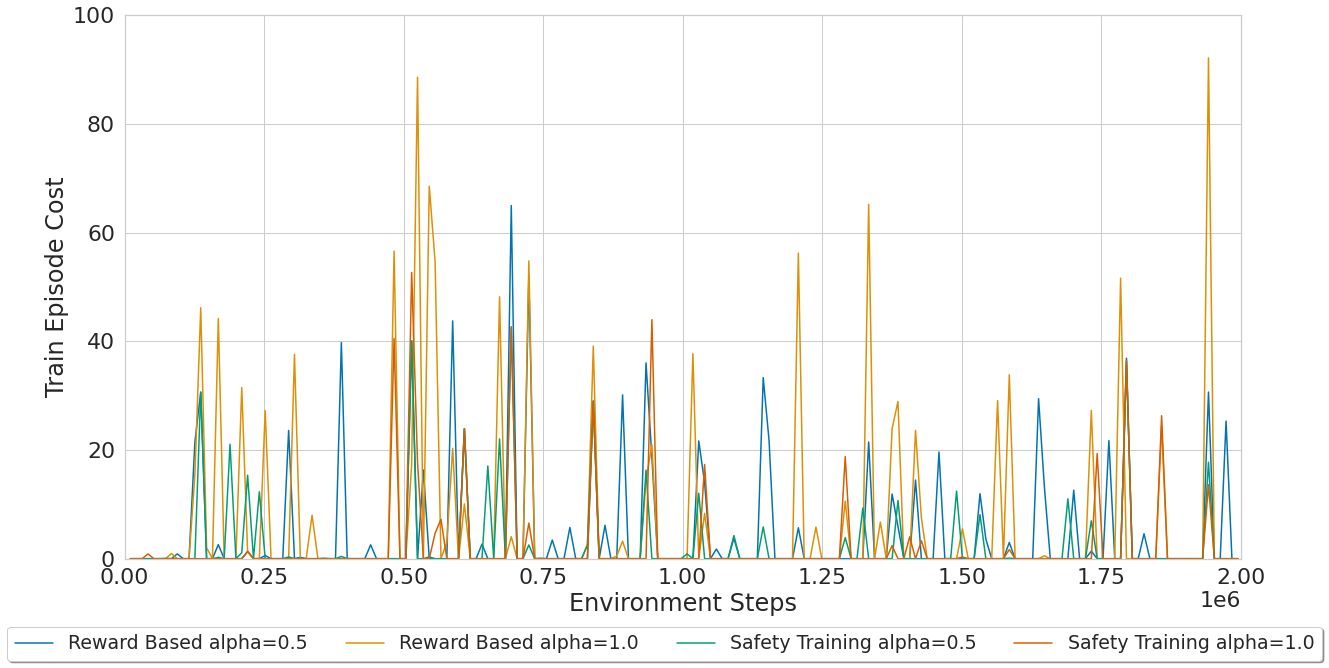
\includegraphics[width=\textwidth]{images/results/push-barrier-drq/cost.png}
    \caption[The episode cost from the FetchPushBarrier pixel experiments.]{The episode cost from the FetchPushBarrier pixel experiments. The FetchPushBarrier environment was trained with the reward based approach as well as the safety training.}
    \label{fig:results:barrier-drq-cost}
\end{figure}

\begin{figure}
    \centering
    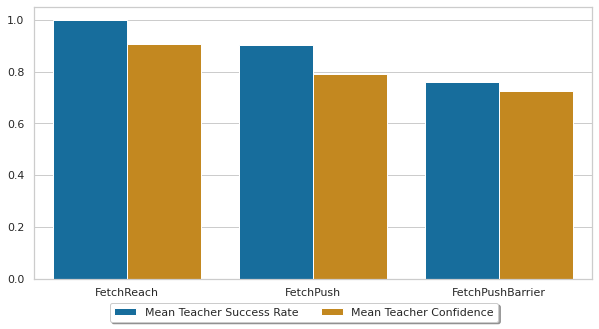
\includegraphics[width=\textwidth]{images/results/ensemble_combined_bar.png}
    \caption[Comparison of the mean success rate and confidence of the teachers.]{Comparison of the mean success rate and confidence of the teachers. For each environment, all three agents that form the ensemble teacher where evaluated on 1000 episodes, to calculate the mean success rate. To calculate the mean confidence, first the best agent of each ensemble, with regards to the success rate, was selected. This agent was evaluated again on 1000 episodes. The environment was initialized with the same seed. For each action, the confidence was calculated using all three agents. The mean of the confidence of all actions is shown here.}
    \label{fig:results:barrier-drq-ensemble-bar}
\end{figure}
\chapter{Conclusion}
\label{ch:Conclusion}

This work had two goals. The first goal was to introduce a teacher to the reinforcement learning framework. The second was to develop new algorithms to train RL agents that safely interact with their environment.

The teacher was introduced with the preference reward algorithm, a reward shaping technique that combines the reward signal from the environment with a new reward function for the teacher. The teacher was defined as a function that maps a state to an action and a confidence about the quality of this action. The teachers action is then compared to the students action using the mean square error, to form the teacher reward. 

For the second goal, we utilized a safety critic. Similar to the reward critic from SAC, the safety critic is trained to estimate the expected cost for the remainder of the episode. Based on the safety critic we proposed to new approaches and compared them to an established reward based approach that deducts the cost from the reward when training the agent. The two safety critic based approaches are safety training and safety evaluation. The safety training algorithm changes the training objective of SAC, to optimize the reward and cost together. In contrast, the safety evaluation algorithm does not change the training. The goal with this algorithm was not to reduce the cost during training, but to learn how to avoid cost during evaluation. To do so, we utilized the stochastic nature of SAC policies to draw multiple actions from the policy and execute the one with lowest cost.

Afterwards we evaluated the three algorithms on two environments form the OpenAI Gym robotics environments as well as a custom environment. The two environment from OpenAI Gym were FetchReach and FetchPush. Based on the FetchPush environment we developed the FetchPushBarrier environment, where the object and the target are always separated by a barrier, the agent has to move the object around.

On the FetchReach environment, we saw that adding a teacher lead to improvements in the success rate when training SAC using pixels and also when adding an autoencoder as an auxiliary loss. When using DrQ to improve the performance of SAC pixel, the agent was able to solve the FetchReach environment without the help of teacher. However, with a teacher we were able to significantly improve the sample efficiency.

For the experiments on the FetchPush environment, we only trained agents with DrQ, since only those were able to reliably solve the FetchReach environment. We saw that an agent trained without the teacher was not able to solve the environment. We then continued to train multiple agents with different values for $\alpha$, the parameter that marks the importance of the teacher. We saw that only trusting the teacher and not using the environment reward at all did not lead to the best results. With an $\alpha$ value of $0.5$ we achieved the best results. We achieved similar results with an adaptive $\alpha$. A function that reduces the $\alpha$ value when the environment reward increases, indicating that the agent learned something.

On the FetchPushBarrier environment, we first trained agents using the full state information, to evaluate the safety training and safety evaluation algorithms. We saw that agents trained with the safety training algorithm were able to outperform the agents trained with the reward based approach we used to compare our new algorithms to. With the safety, training we saw similar, but slightly better success rates, as well as significantly lower episode costs. The agents trained using the safety evaluation algorithm, however, lacked behind, both in the success rate and the episode costs. While the safety evaluation was able to reduce the episode costs in contrast to not using it, the costs are still much higher than using the reward based approach or the safety training algorithm.

Lastly, we performed experiments on the FetchPushBarrier environment using high dimensional image observations. We were not able to reliably solve the task with any configuration we tried. The configuration varied in the safety algorithm we used, as well as the $\alpha$ value. However, we saw that the agents did learn to move the object and even move it around the barrier. We suspect that this is due to the lower quality of the teacher when compared to the teachers of the FetchReach and FetchPush environment. We leave it up to future work to show if an improved teacher can lead to better performance on the FetchPushBarrier environment using high dimensional image observations.

Overall, we saw significant improvements in the sample efficiency or success rate on the FetchReach and FetchPush environments when using the teacher. We were not able to solve the FetchPushBarrier environment when using pixel observations, even with a teacher. However, it unclear if this due to the difficulty of the environment or the fact that the teacher for the FetchPushBarrier environment is significantly worse than the teachers for the other environments. This leaves room for future work to explore the performance on the FetchPushBarrier environment with an improved teacher. A possible solution could be as simple as improving the performance of SAC state on the FetchPushBarrier environment. This could be done for example by using a hindsight experience replay buffer \cite{andrychowiczHindsightExperienceReplay2018}.

In the following we will propose further improvements and experiments that can be explored in future work. Similar to the improved ensemble teacher mentioned above, other teachers could improve the performance. This includes classic control methods like trajectory planners as well as human based teachers. The benefit of these teachers is that they are easier to use in real world scenarios, where it might not be viable to first train multiple agents using the state space. However, these teachers require a new approach to measure the confidence in the actions.

Other improvement we see are in the choice of the parameter $\alpha$. In this work we either set a fixed value or used a linear function based on the environment reward. The first step could be to try different functions that for example decrease the value faster as the environment reward increases. Also another metric could be used to measure how much the agent has learned already and lower the $\alpha$ value accordingly. Another possibility is to directly optimize the $\alpha$ value, similar to the temperature in SAC that defines the importance of the entropy in contrast to the reward. As described in section \ref{sec:results:fetch-push}, an adaptive $\alpha$ can lead to lower preference rewards even when the agent performs better with regards to the environment reward. With off-policy RL algorithms this is not ideal for training. We see a possible solution to this problem by storing both the environment and the teacher reward in the replay buffer. The preference reward is then calculated only when it is needed with the current $\alpha$ value. However, we leave the evaluation of this possible solution for future work.

The most drastic improvement we propose is the combination of the preference reward algorithm with model base RL. In model based RL, a dynamics model is learned to predict the next state of the environment before an action is executed. The learned dynamics model could be used to predict the effect of the teachers action and therefore measure the quality. The importance of the teacher can then be set according to the predicted quality.

Finally, it would be interesting to see the impact of the preference reward algorithm on experiments with real robots. As stated above, it is probably required to utilize a different teacher to the ensemble teacher, used in this work, to avoid the need to train multiple RL agents. The ensemble teacher would also require a lot of additional sensors to measure the state space we had available in the simulation.


%% --------------------
%% |   Bibliography   |
%% --------------------

%% Add entry to the table of contents for the bibliography
\printbibliography[heading=bibintoc]

%% ----------------
%% |   Appendix   |
%% ----------------
\appendix
%%% LaTeX2e class for student theses
%% sections/apendix.tex
%% 
%% Karlsruhe Institute of Technology
%% Institute for Program Structures and Data Organization
%% Chair for Software Design and Quality (SDQ)
%%
%% Dr.-Ing. Erik Burger
%% burger@kit.edu
%%
%% Version 1.3.5, 2020-06-26

\iflanguage{english}
{\chapter{Appendix}}    % english style
{\chapter{Anhang}}      % german style
\label{chap:appendix}


%% -------------------
%% | Example content |
%% -------------------
\section{First Appendix Section}
\label{sec:appendix:FirstSection}
		
\setcounter{figure}{0}
		
\begin{figure} [ht]
  \centering
  \caption{A figure}
  \label{fig:anotherfigure}
\end{figure}


\dots
%% ---------------------
%% | / Example content |
%% ---------------------

\end{document}
